\documentclass[11pt]{article}

\usepackage[T1]{fontenc}
\usepackage[utf8]{inputenc}
\usepackage{lmodern}
\usepackage{microtype}
\usepackage[a4paper,margin=1.08in]{geometry}
\usepackage{amsmath,amssymb,amsthm,mathtools,bm}
\usepackage{mathrsfs}
\usepackage{booktabs,array,longtable}
\usepackage{enumitem}
\usepackage{xcolor}
\usepackage{tikz}
\usepackage{pgfplots}
\usepackage{hyperref}
\usepackage{cleveref}
\usepackage{fancyhdr}
\usepackage{lastpage}

\pgfplotsset{compat=1.18}
\usetikzlibrary{arrows.meta,positioning,calc,decorations.pathreplacing}

\definecolor{navy}{RGB}{25,48,85}
\definecolor{teal}{RGB}{26,111,112}
\definecolor{rust}{RGB}{151,67,42}
\definecolor{lightgray}{RGB}{245,247,249}
\definecolor{midgray}{RGB}{90,98,108}

\hypersetup{
  colorlinks=true,
  linkcolor=navy,
  citecolor=teal,
  urlcolor=rust,
  pdftitle={A Squared-Complex Framework for Square-Prefix Mobius Sums},
  pdfauthor={Fred Viole, OVVO Labs}
}

\pagestyle{fancy}
\fancyhf{}
\fancyhead[L]{\small Squared-complex square-prefix M\"obius sums}
\fancyhead[R]{\small Fred Viole}
\fancyfoot[C]{\small \thepage\ of \pageref{LastPage}}
\setlength{\headheight}{14pt}

\setcounter{tocdepth}{2}
\setcounter{secnumdepth}{3}
\setlist[itemize]{leftmargin=1.5em,itemsep=0.25em,topsep=0.35em}
\setlist[enumerate]{leftmargin=1.7em,itemsep=0.3em,topsep=0.35em}
\allowdisplaybreaks
\raggedbottom
\emergencystretch=2em
\widowpenalty=10000
\clubpenalty=10000
\displaywidowpenalty=10000

\newtheorem{theorem}{Theorem}[section]
\newtheorem{proposition}[theorem]{Proposition}
\newtheorem{lemma}[theorem]{Lemma}
\newtheorem{corollary}[theorem]{Corollary}
\newtheorem{conjecture}[theorem]{Open theorem}
\theoremstyle{definition}
\newtheorem{definition}[theorem]{Definition}
\newtheorem{remark}[theorem]{Remark}
\newtheorem{example}[theorem]{Example}
\newtheorem{caution}[theorem]{Caution}

\crefname{conjecture}{open theorem}{open theorems}
\Crefname{conjecture}{Open theorem}{Open theorems}

\newcommand{\eps}{\varepsilon}
\newcommand{\Pplus}{P^{+}}
\newcommand{\1}{\mathbf{1}}
\newcommand{\vect}[1]{\bm{#1}}
\newcommand{\ip}[2]{\left\langle #1,#2\right\rangle}
\newcommand{\norm}[1]{\left\lVert #1\right\rVert}
\newcommand{\R}{\mathbb{R}}
\newcommand{\N}{\mathbb{N}}
\newcommand{\Z}{\mathbb{Z}}
\newcommand{\C}{\mathbb{C}}
\newcommand{\Repart}{\operatorname{Re}}
\newcommand{\Impart}{\operatorname{Im}}
\newcommand{\card}{\operatorname{card}}

\newcommand{\statusbox}[2]{%
\begin{center}
\fcolorbox{#1}{lightgray}{\parbox{0.91\textwidth}{\small\textbf{#2}}}
\end{center}}

\newcommand{\leanxref}[3]{%
  \par\smallskip
  {\small\noindent\textcolor{teal}{\textbf{#1:}}\par
  \noindent\href{#3}{\nolinkurl{#2}}\par}
  \smallskip
}

\title{\vspace{-1.5em}\textbf{A Squared-Complex Framework for Square-Prefix M\"obius Sums}\\[0.45em]
\large Exact arithmetic, canonical cofactor geometry, lifetime refinement, and the elementary RH bridge}
\author{Fred Viole\\OVVO Labs}
\date{August 2026}

\begin{document}
\maketitle

\begin{abstract}
This paper develops an exact geometric framework for square-prefix values of the Mertens function.  At the complete cutoff
\[
 X_n=(n+1)^2-1,
\]
a squarefree integer cannot contain two prime factors larger than $n+1$.  This gives the exact smooth--transport decomposition
\[
 S_n=M(X_n)=A_n-T_n.
\]
Each squarefree source $m>1$ has a unique canonical factorization
\[
 q_m=\Pplus(m),\qquad c_m=\frac{m}{q_m},
\]
and the squared-complex point
\[
 \left(\frac{c_m+q_m}{2}+i\frac{q_m-c_m}{2}\right)^2
 =m+i\frac{q_m^2-c_m^2}{2}
\]
records the source integer and its canonical factor imbalance simultaneously.  Fixed cofactors trace explicit parabolas, the square-prefix cutoff is vertical, and the square-root smoothness cutoff is a moving parabola whose intersection with the $c$-curve occurs exactly at $q=R$.

The largest-prime parametrization has a sharp endpoint support law that is useful throughout the paper.  If $m\le x$ and $\Pplus(m)>\lfloor x/2\rfloor$, then the canonical cofactor is $c_m=1$ and $m$ itself is prime.  Equivalently, every composite $m\le x$ satisfies
\[
 \Pplus(m)\le\lfloor x/2\rfloor.
\]
Thus the $c=1$ prime fibre is the entire extreme-largest-prime population, while every genuine product fibre has $c\ge2$ and largest prime at most $\lfloor x/2\rfloor$.

For a fixed height threshold $\Lambda>0$, low canonical height has uniformly bounded occupancy in each square block, giving the unconditional bound $|S_N^{\mathrm{low}}(\Lambda)|\ll_\Lambda N$.  A lifetime refinement splits the high population into currently active survivors and completed deaths.  The death increments are supported on a bounded-width integer window in the doubled height $|q^2-c^2|$; divisor bounds imply subpolynomial death increments and an RH-scale local-energy bound for the accumulated death mass.  Consequently the unresolved square-block cancellation may be placed entirely on the active survivor operator
\[
 Z_\Lambda(t)=-\sum_c\mu(c)\,\mathcal K_{\Lambda,t}(c),
\]
where $\mathcal K_{\Lambda,t}(c)$ counts canonical primes $q$ with $cq\le (t+1)^2-1$ and $2\Lambda t<|q^2-c^2|$.

The paper proves the exact arithmetic and geometric reductions, the low-height bound, and the death-process divisor-window estimate.  The remaining power-saving estimate for the signed survivor, equivalently the native high-sector square-prefix estimate, is stated explicitly as an open theorem.  The accompanying Lean development machine-checks the exact finite identities and elementary estimates.  No project axiom and no unconditional proof of the Riemann Hypothesis is claimed.
\end{abstract}

\statusbox{navy}{Status convention.  Results labelled theorem, proposition, lemma, or corollary are proved from the stated definitions or standard cited results.  Numerical values are finite computations.  Statements labelled ``Open theorem'' are the remaining analytic obligations and are not asserted as established.}
\newpage
\tableofcontents
\newpage
%======================================================================

\section{Introduction}
\label{sec:introduction}
%======================================================================

The choice of square prefixes is not cosmetic.  It gives a cutoff with an exact square root, which turns a complicated smoothness condition into a clean one-large-prime decomposition.  The squared complex coordinate is then chosen because it records the product and factor imbalance at the same time.

Set
\[
 X_n=(n+1)^2-1,\qquad S_n=M(X_n).
\]
Why stop immediately before a square?  Because if $m<R^2$ is squarefree, it cannot contain two prime factors larger than $R$.  Every source is therefore either already $R$-smooth or has a unique representation
\[
 m=cq,\qquad c<R<q,
\]
with $q$ prime.  This gives the exact identity
\[
 S_n=A_n-T_n.
\]
The identity is elementary; the difficult question is why the two much larger terms $A_n$ and $T_n$ track each other so closely.

The geometry is designed to make that question visible.  For the factor pair $cq=m$, define
\[
 a=\frac{c+q}{2},\qquad b=\frac{q-c}{2}.
\]
Then
\[
 (a+bi)^2=m+i\frac{q^2-c^2}{2}.
\]
The real coordinate remembers the integer $m$, while the imaginary coordinate measures how uneven the factor pair is.  Fixed cofactors become parabolas.  The complete prefix is cut out by a vertical line.  Smoothness is cut out by a second moving parabola.  A source first enters the prefix, then spends time in the transport region, and finally becomes smooth when the moving boundary reaches its largest prime factor.

This viewpoint separates three logically different mechanisms:
\begin{enumerate}[leftmargin=1.7em,itemsep=0.35em]
\item \emph{exact bookkeeping}: the transport-to-smooth crossing cancels identically in $A-T$;
\item \emph{geometric dilution}: the quadratic map expands area by order $n^2$ at square scale $n$;
\item \emph{analytic cancellation}: the remaining high-height contribution must be controlled through one signed Gram form, including its off-diagonal terms.
\end{enumerate}
The first two are proved here.  The third is the central open estimate.  The coordinate change does not prove cancellation by itself; it identifies the correct state space, scale, and interaction that a proof must control.

The classical criterion this program targets is
\begin{equation}\label{eq:classical-rh-criterion}
 \mathrm{RH}
 \quad\Longleftrightarrow\quad
 M(x)=O_{\eps}\!\left(x^{1/2+\eps}\right)
 \quad\text{for every }\eps>0;
\end{equation}
see, for example, \cite[Ch.~14]{titchmarsh} or \cite{montgomery-vaughan}.  The purpose of the square-block coordinate change is not to assume cancellation in $M(x)$, but to relocate the entire unresolved content of \cref{eq:classical-rh-criterion} onto one explicit finite signed operator, isolated from the exact geometric bookkeeping that surrounds it.

The main exact results are summarized below.

\begin{theorem}[Exact square-root decomposition]
\label{thm:intro-decomposition}
For $R_n=n+1$ and $X_n=R_n^2-1$, define
\begin{align*}
 A_n&:=\sum_{\substack{m\le X_n\\\Pplus(m)\le R_n}}\mu(m),\\
 T_n&:=\sum_{c<R_n}\mu(c)
 \left[
 \pi\!\left(\left\lfloor\frac{X_n}{c}\right\rfloor\right)-\pi(R_n)
 \right].
\end{align*}
Then
\[
 \boxed{S_n=A_n-T_n.}
\]
\end{theorem}

\begin{theorem}[Squared-space recovery]
\label{thm:intro-recovery}
Let $w=x+iy$ be generated by a positive factor pair $cq=x$ through
\[
 y=\frac{q^2-c^2}{2}.
\]
With $\rho=|w|$,
\[
 \boxed{c^2=\rho-y,\qquad q^2=\rho+y.}
\]
Hence the squared point determines the ordered factor pair exactly.
\end{theorem}

\begin{theorem}[Cofactor-curve cutoff intersection]
\label{thm:intro-intersection}
For fixed $c>0$, put
\[
 \gamma_c(x)=\frac{x^2-c^4}{2c^2}.
\]
At cutoff $R>0$, put
\[
 \Gamma_R(x)=\frac{R^4-x^2}{2R^2}.
\]
Then
\[
 \boxed{\gamma_c(x)=\Gamma_R(x)\iff x=cR.}
\]
The curves meet orthogonally at their intersection.  At an arithmetic point $x=cq$, the sign of $\gamma_c(cq)-\Gamma_R(cq)$ is the sign of $q-R$.
\end{theorem}

\begin{theorem}[Exact channel telescoping]
\label{thm:intro-telescoping}
As $R$ increases, a canonical point enters the prefix at $R=\sqrt{cq}$ and crosses from transport to smooth at $R=q$.  The signed mass crossing the moving parabola appears with opposite signs in the increments of $A$ and $-T$.  Therefore all internal channel transfers cancel from the increment of $A-T$; only points entering the new square strip remain.
\end{theorem}

\begin{theorem}[Low-height clustering and lifetime]
\label{thm:intro-low}
Let $m=cq\in B_n$ be canonical and let
\[
 Y_m=\frac{q^2-c^2}{2}.
\]
Then, for $H\ge0$,
\[
 \#\{m\in B_n:|Y_m|\le H\}
 \le\left\lfloor\frac{H}{n}\right\rfloor,
\]
and the count is zero when $H=n$.  For odd sources the bound improves to
$\lfloor H/(2n)\rfloor$.
If $Y_m>0$, the transport lifetime satisfies
\[
 L(m)\le\frac{2Y_m}{q}.
\]
Consequently, for fixed $\Lambda$, the canonical points with $|Y_m|\le\Lambda n$ have uniformly bounded block occupancy, and the transport members have uniformly bounded lifetime.
\end{theorem}

\begin{theorem}[Elementary canonical pointwise criterion]
\label{thm:intro-canonical-HS}
Fix $\Lambda>0$.  Extend the harmless conventions $\Pplus(1)=1$, $c_1=1$, and $Y_1=0$.  For the square block $B_j=[j^2,(j+1)^2)$ define
\[
 d_j^{\mathrm{high}}(\Lambda)
 :=
 \sum_{\substack{m\in B_j\\|Y_m|>\Lambda j}}\mu(m),
 \qquad
 S_N^{\mathrm{high}}(\Lambda)
 :=\sum_{0\le j\le N}d_j^{\mathrm{high}}(\Lambda).
\]
Then the following are equivalent:
\begin{enumerate}[label=\textup{(\roman*)},leftmargin=2.2em,itemsep=0.25em]
\item the Riemann Hypothesis;
\item for every $\eps>0$,
\begin{equation}
 \boxed{
 |S_N^{\mathrm{high}}(\Lambda)|^2
 \ll_{\eps,\Lambda}N^{2+\eps};
 }
 \tag{PHS}
 \label{eq:intro-canonical-PHS}
\end{equation}
\item for every $\eps>0$ and $1\le H\le N$,
\begin{equation}
 \sum_{n=N}^{N+H-1}|S_n^{\mathrm{high}}(\Lambda)|^2
 \ll_{\eps,\Lambda}HN^{2+\eps}.
 \tag{HS}
 \label{eq:intro-canonical-HS}
\end{equation}
\end{enumerate}
The equivalence uses only the exact low/high recombination, the elementary low-sector bound, square-endpoint interpolation, and the classical Mertens criterion.  The implication \textup{(ii)}$\Rightarrow$\textup{(iii)} follows from $N+h<2N$; the reverse implication is the single choice $H=1$.
\end{theorem}

\begin{theorem}[Quadratic conformal expansion]
\label{thm:intro-jacobian}
The map
\[
 \Phi(c,q)=\left(cq,\frac{q^2-c^2}{2}\right)
\]
has
\[
 D\Phi(c,q)^{\mathsf T}D\Phi(c,q)
 =(c^2+q^2)I,
\]
and
\[
 \det D\Phi(c,q)=c^2+q^2\ge2cq.
\]
At square scale $cq\asymp n^2$, lengths expand by at least order $n$ and areas by at least order $n^2$.
\end{theorem}

\begin{theorem}[Exact dyadic cell compression]
\label{thm:intro-dyadic-cell}
For every $k\ge0$,
\[
 \boxed{
 \bigl(\mu(4k+1),\mu(4k+2),\mu(4k+3),\mu(4k+4)\bigr)
 =\bigl(\mu(4k+1),-\mu(2k+1),\mu(4k+3),0\bigr).
 }
\]
Consequently the complete-cell scalar is
\[
 \boxed{C_k=\mu(4k+1)-\mu(2k+1)+\mu(4k+3).}
\]
Among the three active slots $4k+1,4k+2,4k+3$, exactly one is divisible by $3$; the affected slot is $4k+3,4k+2,4k+1$ according as $k\equiv0,1,2\pmod3$.
\end{theorem}

\begin{theorem}[Exact small-modulus quadratic resonance]
\label{thm:intro-prime-square-24}
For every prime $q>3$,
\[
 \boxed{q^2\equiv1\pmod{24}.}
\]
Hence, for every integer $m$ and every prime interval containing no $2$ or $3$,
\[
 \boxed{
 \sum_{Q<q\le2Q\atop q\ {\rm prime}}
 e\!\left(\frac{m q^2}{24}\right)
 =e\!\left(\frac m{24}\right)
 \bigl(\pi(2Q)-\pi(Q)\bigr).
 }
\]
Equivalently, the quadratic prime phase is perfectly coherent at every
$\alpha=m/12$.  More generally, for $\alpha=a/r$, the rational phase
$e(aq^2/(2r))$ is periodic modulo $2r$; the correct reduced-residue model is therefore formed over $(\mathbb Z/2r\mathbb Z)^\times$.
\end{theorem}

The remaining theorem is the pointwise inequality \eqref{eq:intro-canonical-PHS}.  The local estimate \eqref{eq:intro-canonical-HS} is an exact equivalent.  No claim is made that the coordinate change alone supplies cancellation; it identifies the native arithmetic quantity, the correct scale, and the signed interaction that must be controlled.

%======================================================================

\section{Square prefixes and the arithmetic decomposition}
\label{sec:arithmetic}
%======================================================================

The square-root cutoff is the arithmetic hinge of the paper.  Before introducing geometry, we isolate the exact decomposition that the geometry is meant to explain.  The largest-prime cofactor construction used throughout extends the canonical factorization framework developed in \cite{viole-complex}.

Define the complete square block
\begin{equation}
 B_n:=\{m\in\N:n^2\le m<(n+1)^2\},
 \label{eq:block}
\end{equation}
the square-root cutoff
\begin{equation}
 R_n:=n+1,
 \label{eq:Rn}
\end{equation}
and the complete-prefix endpoint
\begin{equation}
 X_n:=R_n^2-1=(n+1)^2-1.
 \label{eq:Xn}
\end{equation}
The square-prefix Mertens value is
\begin{equation}
 S_n:=M(X_n)=\sum_{m\le X_n}\mu(m).
 \label{eq:Sn}
\end{equation}
Because $\mu(R_n^2)=0$ for $R_n>1$, one may equally write $S_n=M(R_n^2)$.

Write $\Pplus(m)$ for the largest prime factor of $m$, with $\Pplus(1)=1$.

\begin{definition}[Smooth and transport terms]
\label{def:AT}
Define
\begin{align}
 A_n
 &:={\sum}_{\substack{1\le m\le X_n\\\Pplus(m)\le R_n}}\mu(m),
 \label{eq:An}\\
 T_n
 &:={\sum}_{1\le c<R_n}\mu(c)
 \left[
 \pi\!\left(\left\lfloor\frac{X_n}{c}\right\rfloor\right)-\pi(R_n)
 \right].
 \label{eq:Tn}
\end{align}
\end{definition}

\begin{lemma}[One-large-prime closure]
\label{lem:one-large}
Let $m\le R^2-1$ be squarefree.  If $\Pplus(m)>R$, then there is a unique factorization
\begin{equation}
 m=cq,
 \qquad
 1\le c<R<q,
 \qquad
 q\text{ prime},
 \label{eq:one-large}
\end{equation}
where $q=\Pplus(m)$.  Moreover,
\begin{equation}
 \mu(m)=-\mu(c).
 \label{eq:mobius-peel}
\end{equation}
\end{lemma}

\begin{proof}
Put $q=\Pplus(m)$ and $c=m/q$.  If $c\ge R$, then $m=cq>R^2$, contrary to $m\le R^2-1$.  Since $m$ is squarefree, $q\nmid c$ and $\mu(cq)=-\mu(c)$.  Uniqueness follows from the largest-prime choice.
\end{proof}
\leanxref{Lean support}{canonical largest-prime and cofactor arithmetic}{https://github.com/OVVO-Financial/square-block-mobius/blob/main/lean/RHLean/Analysis/CanonicalHighSectorCore.lean}

\begin{proof}[Proof of \cref{thm:intro-decomposition}]
Partition the squarefree $m\le X_n$ according to whether $\Pplus(m)\le R_n$ or $\Pplus(m)>R_n$.  The first population contributes $A_n$.  By \cref{lem:one-large}, the second population is uniquely $m=cq$ with $c<R_n<q$, and each source has weight $-\mu(c)$.  The total second contribution is therefore $-T_n$.
\end{proof}

\begin{corollary}[Elementary smooth--transport RH inequality]
\label{cor:elementary-AT-RH}
The Riemann Hypothesis is equivalent to either of the following square-prefix estimates:
\begin{align}
 |A_N-T_N|^2&\ll_\eps N^{2+\eps},
 \label{eq:elementary-AT-squared}\\
 |A_N-T_N|&\ll_\eps N^{1+\eps}.
 \label{eq:elementary-AT-linear}
\end{align}
Here and below the two exponent conventions are equivalent after renaming $\eps$.
\end{corollary}

\begin{proof}
By \cref{thm:intro-decomposition}, $A_N-T_N=M((N+1)^2-1)$.  The classical Mertens criterion \cref{eq:classical-rh-criterion} \cite{titchmarsh,montgomery-vaughan} gives the estimates under RH.  Conversely, every $x$ lies within one square block of an endpoint $(N+1)^2-1$, and $|\mu(m)|\le1$, so the endpoint estimate interpolates to $M(x)\ll_\eps x^{1/2+\eps}$.
\end{proof}

\begin{remark}[Why this is the most elementary total formulation]
The inequality \cref{eq:elementary-AT-linear} contains no shell, window, covariance, probability space, or operator.  It asks only that the two exact cumulative arithmetic terms in $S_N=A_N-T_N$ agree to square-root scale.  The high-sector formulation introduced later removes the part of this agreement already forced by elementary geometry.
\end{remark}

\subsection{The largest-prime cofactor identity}
\label{subsec:central-identity}

For $c\ge1$, define the prime-tail counting function
\begin{equation}
 \Pi_c(x)
 :=
 \#\left\{
 q\text{ prime}:
 \Pplus(c)<q\le\left\lfloor\frac{x}{c}\right\rfloor
 \right\}.
 \label{eq:Pi-c}
\end{equation}
Equivalently,
\begin{equation}
 \Pi_c(x)
 =
 \left(
 \pi\!\left(\left\lfloor\frac{x}{c}\right\rfloor\right)
 -\pi(\Pplus(c))
 \right)_{+},
 \label{eq:Pi-c-positive-part}
\end{equation}
where $(u)_+:=\max\{u,0\}$.  The positive part is essential when
$x/c<\Pplus(c)$.

\begin{theorem}[Exact largest-prime cofactor expansion]
\label{thm:central-M-identity}
For every real $x\ge1$,
\begin{equation}
 \boxed{
 M(x)
 =
 1-\sum_{c\ge1}\mu(c)\Pi_c(x).
 }
 \label{eq:central-M-identity-compact}
\end{equation}
The sum is finite, and separating the prime curve $c=1$ gives
\begin{equation}
 \boxed{
 M(x)
 =
 1-\pi(x)
 -\sum_{2\le c\le x/2}
 \mu(c)
 \left(
 \pi\!\left(\left\lfloor\frac{x}{c}\right\rfloor\right)
 -\pi(\Pplus(c))
 \right)_{+}.
 }
 \label{eq:central-M-identity}
\end{equation}
\end{theorem}

\begin{proof}
Every squarefree $m>1$ has a unique largest prime factor
$q=\Pplus(m)$.  Writing $c=m/q$, one has
\[
 q>\Pplus(c),
 \qquad
 \mu(m)=\mu(cq)=-\mu(c).
\]
Conversely, every pair consisting of a squarefree $c$ and a prime
$q>\Pplus(c)$ produces the squarefree integer $m=cq$ whose largest
prime factor is $q$.  The condition $m\le x$ is exactly $q\le x/c$.
Summing $-\mu(c)$ over these unique pairs proves
\cref{eq:central-M-identity-compact}.  The $c=1$ term is
$-\pi(x)$, because $\Pplus(1)=1$.  No term with $c>x/2$ can occur.
\end{proof}

\begin{theorem}[Extreme largest-prime support and the pure-prime fibre]
\label{thm:extreme-largest-prime}
Let $x\ge2$ and let $1<m\le x$ be an integer.  Put
\[
 q=\Pplus(m),\qquad c=\frac{m}{q}.
\]
If
\begin{equation}
 x<2q,
 \label{eq:extreme-q-condition}
\end{equation}
then
\begin{equation}
 \boxed{c=1,\qquad m=q,}
 \label{eq:extreme-prime-fibre}
\end{equation}
so $m$ is prime.  Equivalently, every composite integer $m\le x$ satisfies
\begin{equation}
 \boxed{\Pplus(m)\le\left\lfloor\frac{x}{2}\right\rfloor.}
 \label{eq:composite-largest-prime-half}
\end{equation}
Moreover, for every genuine canonical product $m=cq\le x$ with $c\ge2$ one also has
\begin{equation}
 \boxed{q\le\left\lfloor\frac{x}{2}\right\rfloor,\qquad
 c\le\left\lfloor\frac{x}{2}\right\rfloor.}
 \label{eq:both-canonical-factors-half}
\end{equation}
Thus canonical sources below $x$ split sharply into the pure prime fibre $c=1$ and genuine product fibres $c\ge2$; the extreme-largest-prime region contains no composites.
\end{theorem}

\begin{proof}
Since $q\mid m$, write $m=cq$ with $c\ge1$.  If $c\ge2$, then
\[
 2q\le cq=m\le x,
\]
contradicting $x<2q$.  Hence $c=1$, so $m=q$ is prime.  The contrapositive gives \cref{eq:composite-largest-prime-half}.  For a genuine product $c\ge2$, the inequality $2q\le cq\le x$ gives the bound on $q$; since every canonical prime satisfies $q\ge2$, the inequality $2c\le cq\le x$ gives the bound on $c$.
\end{proof}
\leanxref{Lean proof}{canonicalCofactor_eq_one_of_endpoint_lt_two_mul_largestPrime; canonicalLargestPrimeFactor_le_half_of_ne_largestPrime}{https://github.com/OVVO-Financial/square-block-mobius/blob/main/lean/RHLean/Analysis/CanonicalExtremePrimeSupport.lean}

\begin{remark}[Two different half-support facts]
The bounds in \cref{thm:extreme-largest-prime} should not be conflated.  The already-used cofactor support $c\le\lfloor x/2\rfloor$ follows from the trivial fact that the canonical prime is at least $2$.  The new extreme-prime statement says that a \emph{composite} source also has $q\le\lfloor x/2\rfloor$.  The only sources whose largest prime exceeds that threshold are the primes themselves on the $c=1$ fibre.
\end{remark}

\begin{remark}[Central analytic engine]
\Cref{eq:central-M-identity} is the exact arithmetic form of the
cofactor-parabola decomposition.  It shows that the Mertens function is
not obtained by proving that the prime curve is small.  The prime curve
$-\pi(x)$ is cancelled by the M\"obius-weighted collection of all
curves $c\ge2$.
\end{remark}

\section{All factor pairs above one integer}
\label{sec:full-fibre}
%======================================================================

A fixed integer has many factor pairs.  This section describes the complete geometric fibre first, so that the later canonical M\"obius point is not confused with the whole factorization geometry.

The factorization geometry and the smooth--transport geometry use the same coordinate map but different point selections.  This distinction is essential.

Fix $N\ge1$ and consider every positive factor pair
\begin{equation}
 uv=N,
 \qquad
 1\le u\le v.
 \label{eq:factor-pair}
\end{equation}
Define the Fermat coordinates
\begin{equation}
 a=\frac{u+v}{2},
 \qquad
 b=\frac{v-u}{2}\ge0.
 \label{eq:full-Fermat}
\end{equation}
Then
\begin{equation}
 u=a-b,
 \qquad
 v=a+b,
 \qquad
 N=a^2-b^2.
 \label{eq:full-recovery}
\end{equation}
The coordinates lie in $\frac12\Z$; they are integers when $u$ and $v$ have the same parity.

Squaring the complex factor gives
\begin{equation}
 (a+bi)^2=N+iY,
 \qquad
 \boxed{Y=2ab=\frac{v^2-u^2}{2}.}
 \label{eq:full-square}
\end{equation}
Thus all factorizations of a fixed $N$ lie on the vertical fibre
\begin{equation}
 \Repart w=N.
 \label{eq:vertical-fibre}
\end{equation}

\subsection{Square-root tests}

Let
\begin{equation}
 w=N+iY,
 \qquad
 \rho=|w|=\sqrt{N^2+Y^2}.
 \label{eq:rho-full}
\end{equation}
Then
\begin{align}
 a^2&=\frac{\rho+N}{2},
 \label{eq:a-square}\\
 b^2&=\frac{\rho-N}{2},
 \label{eq:b-square}\\
 u^2&=\rho-Y,
 \label{eq:u-square}\\
 v^2&=\rho+Y.
 \label{eq:v-square}
\end{align}
Accordingly, a candidate vertical ordinate $Y$ corresponds to an exact factorization if and only if the relevant square and parity conditions hold.  The identity
\begin{equation}
 \sqrt{N^2+Y^2}=a^2+b^2
 \label{eq:hypotenuse}
\end{equation}
is the right-triangle form of the same condition.

\subsection{Admissible intervals}

For a factor pair $u(N/u)=N$ with $1\le u\le\sqrt N$,
\begin{equation}
 a(u)=\frac{u+N/u}{2},
 \qquad
 b(u)=\frac{N/u-u}{2}.
 \label{eq:ab-u}
\end{equation}
Both functions decrease as $u$ increases toward $\sqrt N$.  Therefore the full positive factor fibre satisfies
\begin{align}
 \sqrt N&\le a\le\frac{N+1}{2},
 \label{eq:a-full-range}\\
 0&\le b\le\frac{N-1}{2},
 \label{eq:b-full-range}\\
 0&\le Y\le\frac{N^2-1}{2}.
 \label{eq:Y-full-range}
\end{align}
For integer enumeration one uses $a\ge\lceil\sqrt N\rceil$ with the parity required by $N$.

The upper endpoint corresponds to the trivial factor pair $1\cdot N$.  If the trivial factor is excluded and the smallest permitted odd factor is $3$, then
\begin{align}
 a&\le\frac{N+9}{6},
 \label{eq:a-three}\\
 b&\le\frac{N-9}{6},
 \label{eq:b-three}\\
 Y&\le\frac{N^2-81}{18}.
 \label{eq:Y-three}
\end{align}
These are the nontrivial odd-factor or semiprime-search envelopes.  They are not the universal bounds for the complete factor fibre.

\begin{example}[The fibre $N=309$]
The trivial factor pair $1\cdot309$ gives
\[
 (a,b)=(155,154),
 \qquad
 w=309+47740i.
\]
The nontrivial factorization $3\cdot103$ gives
\[
 (a,b)=(53,50),
 \qquad
 w=309+5300i.
\]
The latter is the highest point allowed by the nontrivial odd-factor condition $u\ge3$, but not the highest point on the full factor fibre.
\end{example}

\begin{figure}[htbp]
\centering
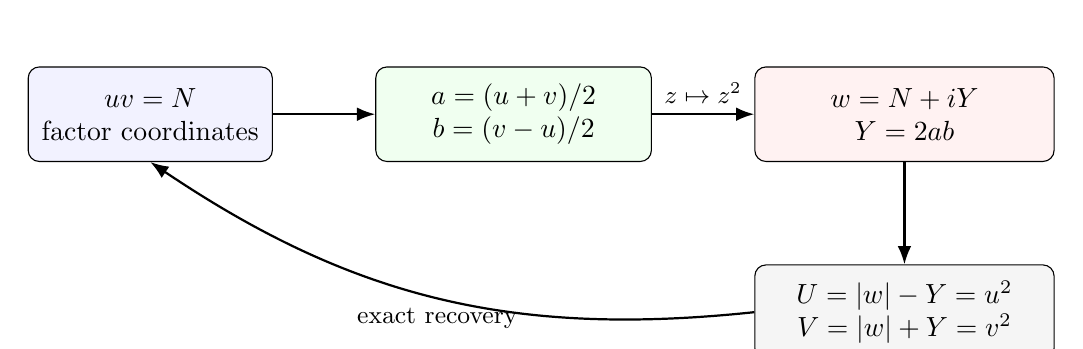
\begin{tikzpicture}[>=Latex,node distance=13mm]
  \node[draw,rounded corners,fill=blue!5,align=center,minimum width=31mm,minimum height=12mm] (factor) {$uv=N$\\factor coordinates};
  \node[draw,rounded corners,fill=green!6,align=center,minimum width=35mm,minimum height=12mm,right=of factor] (fermat) {$a=(u+v)/2$\\$b=(v-u)/2$};
  \node[draw,rounded corners,fill=red!5,align=center,minimum width=38mm,minimum height=12mm,right=of fermat] (square) {$w=N+iY$\\$Y=2ab$};
  \node[draw,rounded corners,fill=gray!8,align=center,minimum width=38mm,minimum height=12mm,below=of square] (null) {$U=|w|-Y=u^2$\\$V=|w|+Y=v^2$};
  \draw[->,thick] (factor) -- (fermat);
  \draw[->,thick] (fermat) -- node[above,font=\small] {$z\mapsto z^2$} (square);
  \draw[->,thick] (square) -- (null);
  \draw[->,thick,bend left=20] (null.west) to node[below,font=\small] {exact recovery} (factor.south);
\end{tikzpicture}
\caption{Equivalent coordinate systems on a complete factor fibre.  The squared coordinates retain the factor pair exactly.}
\label{fig:coordinate-map}
\end{figure}

%======================================================================

\section{The canonical M\"obius geometry}
\label{sec:canonical-cloud}
%======================================================================

The M\"obius decomposition needs one reproducible point per squarefree source.  Choosing the largest prime factor supplies that point and gives a signed height that can be followed across cutoffs.

The smooth--transport decomposition does not use every point on each factor fibre.  It selects one canonical point per squarefree source.

For squarefree $m>1$, define
\begin{equation}
 q_m:=\Pplus(m),
 \qquad
 c_m:=\frac{m}{q_m}.
 \label{eq:canonical-cq}
\end{equation}
Unlike the ordered factor pair in \cref{sec:full-fibre}, the canonical pair is not reordered.  The cofactor $c_m$ may exceed $q_m$.  For example,
\[
 m=30,
 \qquad
 q_m=5,
 \qquad
 c_m=6.
\]
Therefore define the signed Fermat coordinate
\begin{equation}
 a_m:=\frac{c_m+q_m}{2},
 \qquad
 b_m:=\frac{q_m-c_m}{2}\in\frac12\Z,
 \label{eq:signed-Fermat}
\end{equation}
and the canonical squared point
\begin{equation}
 w_m:=(a_m+ib_m)^2
 =m+iY_m,
 \label{eq:canonical-w}
\end{equation}
where
\begin{equation}
 \boxed{Y_m=2a_mb_m=\frac{q_m^2-c_m^2}{2}.}
 \label{eq:signed-Y}
\end{equation}
The sign of $Y_m$ records the order of the canonical factors:
\begin{equation}
 Y_m>0\iff c_m<q_m,
 \qquad
 Y_m<0\iff c_m>q_m.
 \label{eq:Y-sign}
\end{equation}

\subsection{Parameterization by cofactors and primes}

Every squarefree $m>1$ has a unique representation
\begin{equation}
 m=cq,
 \label{eq:cq-general}
\end{equation}
where
\begin{equation}
 \mu(c)\ne0,
 \qquad
 q\text{ is prime},
 \qquad
 q>\Pplus(c).
 \label{eq:canonical-admissibility}
\end{equation}
Conversely, every pair satisfying \cref{eq:canonical-admissibility} produces a squarefree integer $m=cq$ with largest prime factor $q$.  Moreover,
\begin{equation}
 \mu(cq)=-\mu(c).
 \label{eq:canonical-sign}
\end{equation}

Define the canonical index set
\begin{equation}
 \mathscr C
 :=
 \left\{
 (c,q):
 \mu(c)\ne0,
 \ q\text{ is prime},
 \ q>\Pplus(c)
 \right\}.
 \label{eq:canonical-index}
\end{equation}
The squared point cloud is
\begin{equation}
 \mathscr W
 :=
 \left\{
 cq+i\frac{q^2-c^2}{2}:(c,q)\in\mathscr C
 \right\}.
 \label{eq:canonical-cloud}
\end{equation}
The signed point measure is
\begin{equation}
 \nu
 :=
 \delta_1
 -
 \sum_{(c,q)\in\mathscr C}
 \mu(c)\,
 \delta_{\,cq+i(q^2-c^2)/2}.
 \label{eq:signed-measure}
\end{equation}
The atom at $1$ records $\mu(1)=1$.

\begin{example}[A point below the real axis]
For $m=30$, the canonical pair is $(c,q)=(6,5)$, so
\[
 a=\frac{11}{2},
 \qquad
 b=-\frac12,
 \qquad
 w_{30}=30-\frac{11}{2}i.
\]
This point enters a square prefix only after the cutoff already exceeds $q=5$, so it is smooth immediately and never occupies the transport channel.
\end{example}

%======================================================================

\section{Four equivalent coordinate systems}
\label{sec:coordinates}
%======================================================================

Different calculations become simple in different coordinates.  The point is not to multiply notation, but to move between product, factor-gap, norm, and null coordinates without losing information.

Let
\begin{equation}
 w=x+iy
 =cq+i\frac{q^2-c^2}{2},
 \qquad
 \rho:=|w|=\sqrt{x^2+y^2}.
 \label{eq:w-rho}
\end{equation}
Then
\begin{equation}
 \rho=\frac{c^2+q^2}{2}.
 \label{eq:rho-cq}
\end{equation}
The most useful coordinate charts are collected in \cref{tab:coordinates}.

\begin{table}[htbp]
\centering
\caption{Equivalent coordinates for a canonical squared factor point.}
\label{tab:coordinates}
\renewcommand{\arraystretch}{1.35}
\begin{tabular}{>{\raggedright\arraybackslash}p{0.21\textwidth} >{\raggedright\arraybackslash}p{0.31\textwidth} >{\raggedright\arraybackslash}p{0.34\textwidth}}
\toprule
Coordinate system & Definition & Exact inverse information\\
\midrule
Factor coordinates & $(c,q)$ & $m=cq$, $q=\Pplus(m)$\\
Fermat coordinates & $a=(c+q)/2$, $b=(q-c)/2$ & $c=a-b$, $q=a+b$\\
Squared Cartesian & $x=cq$, $y=(q^2-c^2)/2$ & $w=x+iy=(a+ib)^2$\\
Radial-null & $U=\rho-y$, $V=\rho+y$ & $U=c^2$, $V=q^2$, $x^2=UV$\\
Square-root & $a^2=(\rho+x)/2$, $b^2=(\rho-x)/2$ & sign of $b$ is sign of $y$\\
\bottomrule
\end{tabular}
\end{table}

The central identities are
\begin{equation}
 \boxed{
 U:=\rho-y=c^2,
 \qquad
 V:=\rho+y=q^2.
 }
 \label{eq:UV}
\end{equation}
Consequently,
\begin{equation}
 x=\sqrt{UV}=cq,
 \qquad
 y=\frac{V-U}{2}.
 \label{eq:xy-UV}
\end{equation}

These null coordinates linearize the arithmetic cutoffs.  They also make the meaning of $2ab$ exact:
\begin{equation}
 \boxed{Y=2ab=\frac{V-U}{2},}
 \label{eq:Y-null}
\end{equation}
so the imaginary coordinate is half the separation between the squared canonical factors.

%======================================================================

\section{Fixed-cofactor parabolas}
\label{sec:cofactor-curves}
%======================================================================

Once the cofactor is fixed, the canonical points are no longer an unstructured cloud.  They lie on explicit curves, which lets arithmetic transitions be read geometrically.

Fix a positive cofactor $c$ and let $q$ vary.  In squared Cartesian coordinates,
\begin{equation}
 x=cq,
 \qquad
 y=\frac{q^2-c^2}{2}.
 \label{eq:curve-param}
\end{equation}
Eliminating $q=x/c$ gives the cofactor parabola
\begin{equation}
 \boxed{
 \gamma_c(x)
 =\frac{x^2-c^4}{2c^2}.
 }
 \label{eq:gamma-c}
\end{equation}
The canonical point cloud is not the filled region between envelopes.  It is the arithmetic sampling
\begin{equation}
 x=cq,
 \qquad
 q\text{ prime},
 \qquad
 q>\Pplus(c),
 \label{eq:curve-sampling}
\end{equation}
on the family \cref{eq:gamma-c}.

The curve crosses the real axis at
\begin{equation}
 x=c^2.
 \label{eq:curve-axis-cross}
\end{equation}
Points to the right have $q>c$ and positive ordinate; points to the left have $q<c$ and negative ordinate.

The $c=1$ curve is
\begin{equation}
 \gamma_1(x)=\frac{x^2-1}{2}.
 \label{eq:prime-curve}
\end{equation}
Its arithmetic samples are exactly the prime points, since $m=1\cdot q=q$.  It is the outer positive envelope of the complete canonical cloud.  The curve
\begin{equation}
 \gamma_3(x)=\frac{x^2-81}{18}
 \label{eq:three-curve}
\end{equation}
is the first nontrivial odd-cofactor envelope used in semiprime search.

\begin{figure}[htbp]
\centering
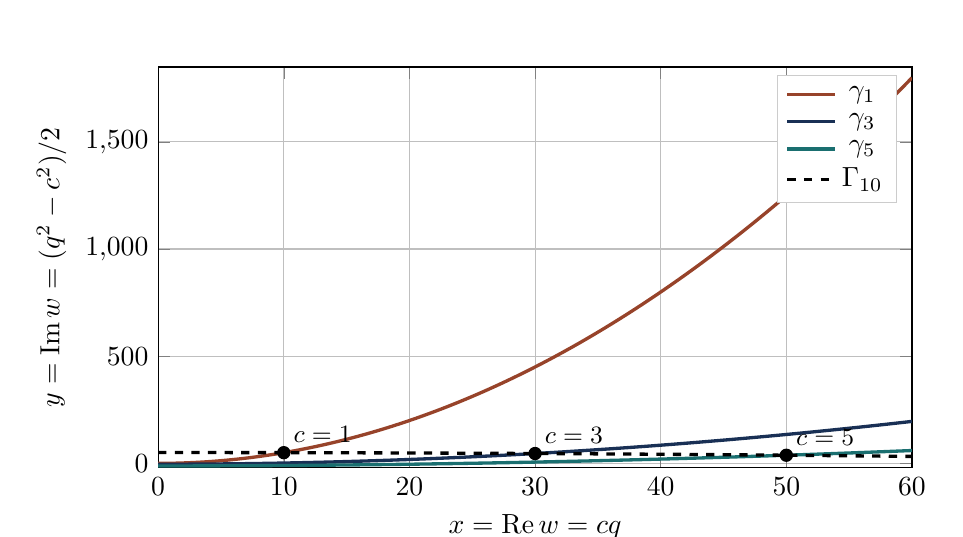
\begin{tikzpicture}
\begin{axis}[
  width=0.92\textwidth,
  height=0.55\textwidth,
  xmin=0,xmax=60,
  ymin=-20,ymax=1850,
  xlabel={$x=\Repart w=cq$},
  ylabel={$y=\Impart w=(q^2-c^2)/2$},
  grid=major,
  legend style={at={(0.98,0.98)},anchor=north east,fill=white,draw=gray!40},
  samples=240,
  domain=0:60,
  clip=true
]
  \addplot[very thick,rust] {(x^2-1)/2};
  \addlegendentry{$\gamma_1$}
  \addplot[very thick,navy] {(x^2-81)/18};
  \addlegendentry{$\gamma_3$}
  \addplot[very thick,teal] {(x^2-625)/50};
  \addlegendentry{$\gamma_5$}
  \addplot[very thick,black,dashed] {(10000-x^2)/200};
  \addlegendentry{$\Gamma_{10}$}
  \addplot[only marks,mark=*,mark size=2.2pt,black] coordinates {(10,49.5) (30,45.5) (50,37.5)};
  \node[anchor=south west,font=\small] at (axis cs:10,49.5) {$c=1$};
  \node[anchor=south west,font=\small] at (axis cs:30,45.5) {$c=3$};
  \node[anchor=south west,font=\small] at (axis cs:50,37.5) {$c=5$};
\end{axis}
\end{tikzpicture}
\caption{Cofactor parabolas $\gamma_c$ and the moving cutoff parabola $\Gamma_R$ for $R=10$.  Each $\gamma_c$ meets $\Gamma_R$ at $x=cR$.  Actual canonical points are discrete prime samples on the curves.}
\label{fig:cofactor-parabolas}
\end{figure}

%======================================================================

\section{Two moving boundaries}
\label{sec:moving-cutoff}
%======================================================================

The decomposition changes with the cutoff.  The goal here is to represent that changing arithmetic classification as motion of two simple boundaries through one fixed point cloud.

Fix $R>0$.  The complete arithmetic prefix is
\begin{equation}
 \mathscr P_R
 :=\{w=x+iy\in\mathscr W:x<R^2\}.
 \label{eq:prefix-region}
\end{equation}
Since $V=q^2=|w|+y$, the smooth condition $q\le R$ is
\begin{equation}
 |w|+y\le R^2.
 \label{eq:smooth-radial}
\end{equation}
Define
\begin{align}
 \mathscr A_R
 &:={\{w\in\mathscr P_R:|w|+\Impart w\le R^2\}},
 \label{eq:A-region}\\
 \mathscr U_R
 &:={\{w\in\mathscr P_R:|w|+\Impart w>R^2\}}.
 \label{eq:U-region}
\end{align}
The prefix is the disjoint union
\begin{equation}
 \mathscr P_R=\mathscr A_R\,\dot\cup\,\mathscr U_R.
 \label{eq:region-partition}
\end{equation}

Solving \cref{eq:smooth-radial} on the boundary gives
\begin{equation}
 \boxed{
 \Gamma_R(x)=\frac{R^4-x^2}{2R^2}.
 }
 \label{eq:Gamma-R}
\end{equation}
Inside the prefix strip $x<R^2$, the smooth region lies below the graph and the transport region lies above it.

In null coordinates, the same regions are even simpler:
\begin{align}
 \mathscr P_R&:\quad UV<R^4,
 \label{eq:prefix-UV}\\
 \mathscr A_R&:\quad UV<R^4,\quad V\le R^2,
 \label{eq:smooth-UV}\\
 \mathscr U_R&:\quad UV<R^4,\quad V>R^2.
 \label{eq:transport-UV}
\end{align}
For a transport point, $UV<R^4<V^2$, so automatically $U<R^2$.  Thus
\begin{equation}
 \mathscr U_R:\quad U<R^2<V,
 \qquad
 UV<R^4.
 \label{eq:transport-null-clean}
\end{equation}
This is exactly $c<R<q$.

\subsection{Intersection with every cofactor curve}

\begin{proposition}[Intersection factorization]
\label{prop:intersection-factorization}
For $c,R>0$,
\begin{equation}
 \gamma_c(x)-\Gamma_R(x)
 =
 \frac{(R^2+c^2)(x^2-c^2R^2)}{2c^2R^2}.
 \label{eq:curve-gap}
\end{equation}
Consequently,
\begin{equation}
 \gamma_c(x)=\Gamma_R(x)
 \iff x=cR.
 \label{eq:curve-intersection}
\end{equation}
At the arithmetic point $x=cq$,
\begin{equation}
 \gamma_c(cq)-\Gamma_R(cq)
 =
 \frac{(R^2+c^2)(q^2-R^2)}{2R^2}.
 \label{eq:point-gap}
\end{equation}
\end{proposition}

The sign is therefore exact:
\begin{align}
 q<R&\iff w_{c,q}\text{ lies below }\Gamma_R,
 \label{eq:below}\\
 q>R&\iff w_{c,q}\text{ lies above }\Gamma_R.
 \label{eq:above}
\end{align}

\begin{proposition}[Orthogonal crossing]
\label{prop:orthogonal-crossing}
At the intersection $x=cR$,
\begin{equation}
 \gamma_c'(cR)=\frac{R}{c},
 \qquad
 \Gamma_R'(cR)=-\frac{c}{R},
 \label{eq:orthogonal-slopes}
\end{equation}
so
\begin{equation}
 \gamma_c'(cR)\Gamma_R'(cR)=-1.
 \label{eq:orthogonal-product}
\end{equation}
Hence each cofactor curve meets the moving cutoff orthogonally.
\end{proposition}

The transition is therefore transverse, never tangent.  A canonical point cannot remain trapped in a thin boundary layer as the cutoff passes its largest prime.

%======================================================================

\section{The moving-region interpretation of $A-T$}
\label{sec:moving-region-AT}
%======================================================================

This section translates the algebraic identity $A-T$ into a geometric partition.  It is the bridge between the original Mertens sum and the later kernel formulation.

Using the signed measure \cref{eq:signed-measure}, define
\begin{equation}
 \mathcal A(R):=\nu(\mathscr A_R),
 \qquad
 \mathcal U(R):=\nu(\mathscr U_R).
 \label{eq:AU-measures}
\end{equation}
At $R=R_n$,
\begin{equation}
 \mathcal A(R_n)=A_n,
 \qquad
 \mathcal U(R_n)=-T_n.
 \label{eq:AU-AT}
\end{equation}
Indeed, the transport points satisfy $c<R_n<q$ and carry signed point mass
\[
 \mu(cq)=-\mu(c).
\]
Therefore
\begin{equation}
 \boxed{
 S_n
 =\nu(\mathscr P_{R_n})
 =\mathcal A(R_n)+\mathcal U(R_n)
 =A_n-T_n.
 }
 \label{eq:geometric-AT}
\end{equation}

Equivalently, define projectors
\begin{align}
 P_R(w)&:=\1_{\{\Repart w<R^2\}},
 \label{eq:P-projector}\\
 Q_R(w)&:=\1_{\{|w|+\Impart w\le R^2\}}.
 \label{eq:Q-projector}
\end{align}
Then
\begin{align}
 \mathcal A(R)&=\int P_RQ_R\,d\nu,
 \label{eq:A-projector}\\
 \mathcal U(R)&=\int P_R(1-Q_R)\,d\nu,
 \label{eq:U-projector}\\
 S(R)&=\int P_R\,d\nu.
 \label{eq:S-projector}
\end{align}
The identity is the pointwise partition
\begin{equation}
 P_R=P_RQ_R+P_R(1-Q_R).
 \label{eq:projector-partition}
\end{equation}

%======================================================================

\section{Entry, transition, and telescoping}
\label{sec:telescoping}
%======================================================================

A source contributes at different times for different reasons.  Separating entry from transition shows which changes are genuine new data and which are internal transfers that cancel.

For a canonical source $m=cq$, define its first square-prefix index
\begin{equation}
 e(m):=\lfloor\sqrt m\rfloor.
 \label{eq:entry-index}
\end{equation}
This is the least $n$ such that $m<R_n^2$.  Define the smoothness-transition index
\begin{equation}
 h(m):=q-1.
 \label{eq:transition-index}
\end{equation}
This is the least $n$ such that $q\le R_n$.

The transport lifetime is
\begin{equation}
 L(m):=(h(m)-e(m))_+.
 \label{eq:lifetime}
\end{equation}
There are two cases:

\begin{enumerate}[leftmargin=1.7em,itemsep=0.3em]
\item If $q>\sqrt m$, equivalently $q>c$ and $Y>0$, then the point enters above the moving parabola and occupies transport for the discrete interval
\[
 e(m)\le n<h(m).
\]
\item If $q\le\sqrt m$, equivalently $q\le c$ and $Y\le0$, then $h(m)\le e(m)$ and the point enters already smooth.  Its transport interval is empty.
\end{enumerate}

Define the pointwise indicators
\begin{align}
 p_n(m)&:=\1_{\{e(m)\le n\}},
 \label{eq:p-indicator}\\
 u_n(m)&:=\1_{\{e(m)\le n<h(m)\}},
 \label{eq:u-indicator}\\
 a_n(m)&:=\1_{\{e(m)\le n,\ h(m)\le n\}}.
 \label{eq:a-indicator}
\end{align}
Then
\begin{equation}
 \boxed{p_n(m)=u_n(m)+a_n(m).}
 \label{eq:temporal-partition}
\end{equation}

\subsection{Why the crossing cancels}

Let $E_n^A$ be the signed mass entering the new vertical strip already below the moving parabola, let $E_n^U$ be the signed mass entering above it, and let $C_n$ be the signed mass crossed by the moving parabola between $R_{n-1}$ and $R_n$.  Then
\begin{align}
 \mathcal A(R_n)-\mathcal A(R_{n-1})
 &=E_n^A+C_n,
 \label{eq:Delta-A}\\
 \mathcal U(R_n)-\mathcal U(R_{n-1})
 &=E_n^U-C_n.
 \label{eq:Delta-U}
\end{align}
Therefore
\begin{equation}
 \boxed{
 S_n-S_{n-1}
 =E_n^A+E_n^U
 =\sum_{m\in B_n}\mu(m).
 }
 \label{eq:Delta-S}
\end{equation}
The entire crossing mass cancels.

\begin{figure}[htbp]
\centering
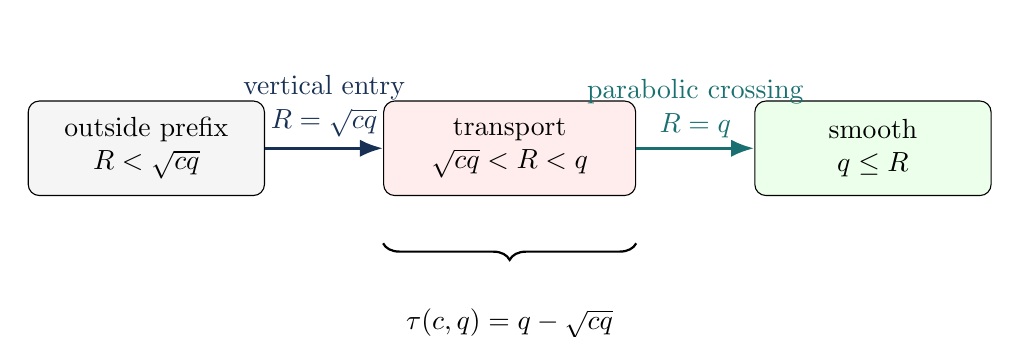
\begin{tikzpicture}[>=Latex,node distance=15mm]
  \node[draw,rounded corners,fill=gray!8,minimum width=30mm,minimum height=12mm,align=center] (out) {outside prefix\\$R<\sqrt{cq}$};
  \node[draw,rounded corners,fill=red!7,minimum width=32mm,minimum height=12mm,align=center,right=of out] (trans) {transport\\$\sqrt{cq}<R<q$};
  \node[draw,rounded corners,fill=green!8,minimum width=30mm,minimum height=12mm,align=center,right=of trans] (smooth) {smooth\\$q\le R$};
  \draw[->,very thick,navy] (out) -- node[above,align=center] {vertical entry\\$R=\sqrt{cq}$} (trans);
  \draw[->,very thick,teal] (trans) -- node[above,align=center] {parabolic crossing\\$R=q$} (smooth);
  \draw[decorate,decoration={brace,amplitude=6pt,mirror},thick] ($(trans.south west)+(0,-6mm)$) -- ($(trans.south east)+(0,-6mm)$) node[midway,below=7mm] {$\tau(c,q)=q-\sqrt{cq}$};
\end{tikzpicture}
\caption{The exact state path of a positive-height canonical point.  The second transition only reallocates signed mass between $-T$ and $A$, so it cancels from the residual increment.}
\label{fig:state-path}
\end{figure}

This is the telescopic nature of the squared coordinate: the point's imaginary height determines when the moving parabola reaches it, while the crossing itself contributes zero to the increment of the total prefix mass.

%======================================================================

\section{Why $2ab$ measures both height and lifetime}
\label{sec:lifetime-law}
%======================================================================

The same imaginary coordinate that measures factor imbalance also measures how long a source remains in transport.  This is the key space--time link in the construction.

Define the signed continuous delay
\begin{equation}
 \tau(c,q):=q-\sqrt{cq}.
 \label{eq:tau}
\end{equation}
It is positive exactly for transport-capable points, zero at $c=q$, and negative for points that enter already smooth.

Put
\begin{equation}
 r:=\frac cq.
 \label{eq:r-ratio}
\end{equation}
Then
\begin{equation}
 Y=\frac{q^2}{2}(1-r^2)
 \label{eq:Y-r}
\end{equation}
and
\begin{equation}
 \tau=q(1-\sqrt r).
 \label{eq:tau-r}
\end{equation}
Since
\begin{equation}
 1-r^2=(1-\sqrt r)(1+\sqrt r)(1+r),
 \label{eq:factor-r}
\end{equation}
we obtain an exact identity.

\begin{theorem}[Exact height--lifetime identity]
\label{thm:exact-height-lifetime}
For every positive pair $(c,q)$,
\begin{equation}
 \boxed{
 Y
 =
 \frac{q\tau}{2}
 \left(1+\sqrt{\frac cq}\right)
 \left(1+\frac cq\right).
 }
 \label{eq:Y-tau-exact}
\end{equation}
Equivalently,
\begin{equation}
 \boxed{
 \tau
 =
 \frac{2Y}
 {q\left(1+\sqrt{c/q}\right)\left(1+c/q\right)}.
 }
 \label{eq:tau-Y-exact}
\end{equation}
\end{theorem}

The sign of $Y$ is therefore exactly the sign of the continuous delay.  On the transport side $0<c/q<1$, the denominator in \cref{eq:tau-Y-exact} lies between $q$ and $4q$, giving
\begin{equation}
 \frac{Y}{2q}
 \le\tau
 \le\frac{2Y}{q}.
 \label{eq:tau-bounds}
\end{equation}
Since
\begin{equation}
 L(m)=q-1-\lfloor\sqrt m\rfloor
 \le q-\sqrt m=\tau(c,q)
 \label{eq:L-tau}
\end{equation}
for transport points,
\begin{equation}
 \boxed{L(m)\le\frac{2Y_m}{q_m}.}
 \label{eq:L-Y}
\end{equation}

In squared-space coordinates, $q=\sqrt{|w|+\Impart w}$, so
\begin{equation}
 L(w)
 \le
 \frac{2(\Impart w)_+}
 {\sqrt{|w|+\Impart w}}.
 \label{eq:L-w}
\end{equation}
A point close to the real axis cannot remain in transport for many prefix steps.

%======================================================================

\section{Exact scale transfer and prime dilation of the transport term}
\label{sec:scale-transfer}
%======================================================================

The decomposition $S_n=A_n-T_n$ is exact but static.  This section records the exact \emph{dynamic} content: the transport term $T_n$ is not an independent object but a prime-weighted image of lower-scale Mertens values, transported through the same $2ab$ geometry that governs entry and smoothness.  Every identity here is finite and unconditional; none of them, by itself, is a bound.

\subsection{Source-resolved entry, smoothness, and transport}

For a squarefree source $m=cq$ with $q=\Pplus(m)$, define the entry and transition indices
\begin{equation}
 e(m):=\lfloor\sqrt m\rfloor,
 \qquad
 h(m):=q-1,
 \label{eq:entry-transition-indices}
\end{equation}
so that at stage $n$ the source has entered the prefix when $e(m)\le n$ and is square-root smooth when $h(m)\le n$.  With source weight $\mu(m)$,
\begin{equation}
 \underbrace{\mu(m)\mathbf 1[e(m)\le n]}_{\text{entered}}
 =\underbrace{\mu(m)\mathbf 1[h(m)\le n]}_{\text{smooth}}
 -\underbrace{\bigl(-\mu(m)\bigr)\mathbf 1[e(m)\le n<h(m)]}_{\text{transport}} .
 \label{eq:entered-smooth-transport}
\end{equation}
Summing \cref{eq:entered-smooth-transport} over every source and every finite stage returns the dynamic recombination
\begin{equation}
 S_n=A_n-T_n,
 \label{eq:dynamic-recombination}
\end{equation}
now realized \emph{atom by atom} rather than only in aggregate.

\subsection{Square-root inversion}

Fix the cutoff $R=R_n$ and set
\begin{equation}
 \iota_R(x):=\frac{R^2}{x}.
 \label{eq:sqrt-inversion}
\end{equation}
It is an involution with the single fixed point $R$, and at radius $R=\sqrt{cq}$ it exchanges the two canonical factors, $\iota_R(c)=q$.  It carries the lower interval $[c,R]$ onto the upper interval $[R,R^2/c]$, whose Euclidean lengths obey the exact scaling
\begin{equation}
 \frac{R^2}{c}-R=\frac Rc\,(R-c).
 \label{eq:inversion-length}
\end{equation}
The normalized ordinate is the exact record of this dilation: writing $\lambda_m=\sqrt{q_m/c_m}$,
\begin{equation}
 \frac{q_m^2-c_m^2}{2c_mq_m}
 =\frac{\lambda_m^2-\lambda_m^{-2}}2,
 \qquad
 \log\lambda_m=\tfrac12\operatorname{asinh}\!\left(\frac{q_m^2-c_m^2}{2c_mq_m}\right).
 \label{eq:twoab-dilation}
\end{equation}
Inversion is a geometric map only; it does not preserve primality, and the prime density must re-enter through an explicit multiplier or discrepancy.

\subsection{The exact $2ab$ scale-transfer identity}

Because every sum defining $T_n$ in \cref{eq:Tn} is finite, the cofactor and prime summations may be interchanged.  Using $q>R_n$ and $X_n<R_n^2$, one has $\lfloor X_n/q\rfloor<R_n$, so each prime-first inner sum is a \emph{complete lower-scale Mertens value}.

\begin{theorem}[Prime-first transport transfer]
\label{thm:transport-primefirst}
For every $n\ge1$,
\begin{equation}
 \boxed{
 T_n
 =\sum_{\substack{R_n<q\le X_n\\ q\ \mathrm{prime}}}
 M\!\left(\left\lfloor\frac{X_n}{q}\right\rfloor\right).
 }
 \label{eq:transport-primefirst}
\end{equation}
The complete high-prime transport population is built entirely from Mertens values strictly below the cutoff.
\end{theorem}

Grouping the primes by the reciprocal coordinate $d=\lfloor X_n/q\rfloor$ places the transfer in lower-triangular form.

\begin{theorem}[Reciprocal prime-dilation formula]
\label{thm:prime-dilation}
For every $n\ge1$,
\begin{equation}
 \boxed{
 T_n=\sum_{1\le d<R_n}K_n(d)\,M(d),
 \qquad
 K_n(d)=\pi\!\left(\left\lfloor\frac{X_n}{d}\right\rfloor\right)
 -\pi\!\left(\max\!\left(R_n,\left\lfloor\frac{X_n}{d+1}\right\rfloor\right)\right).
 }
 \label{eq:prime-dilation}
\end{equation}
The kernel $K_n(d)$ is exactly the prime mass in the square-root-inverted interval $X_n/(d+1)<q\le X_n/d$.  The transport term is thus a fixed lower-triangular prime-dilation operator applied to the Mertens sequence.
\end{theorem}

The same construction mirrors the positive-orientation part of the smooth term.  Splitting $A_n=A_n^++A_n^-$ into the canonical pairs $c<q\le R_n$ and the born-smooth remainder $q\le c$, the mirrored part is again an exact prime transform of lower Mertens values,
\begin{equation}
 A_n^+=-\sum_{q\le R_n}M(q-1),
 \label{eq:A-plus-primeform}
\end{equation}
so the difficult cancellation in $S_n=A_n-T_n$ is not between unrelated objects but between two operators generated by the \emph{same} canonical factor geometry.

\subsection{The baseline discrepancy}

For any deterministic baseline $F$ with $F(R)\ne F(c)$, define the scale multiplier and signed discrepancy of an observable $G$ by
\begin{equation}
 \kappa_F(R,c)=\frac{F(R^2/c)-F(R)}{F(R)-F(c)},
 \qquad
 E_{G,F}(R,c)=\bigl[G(R^2/c)-G(R)\bigr]-\kappa_F(R,c)\bigl[G(R)-G(c)\bigr].
 \label{eq:baseline-discrepancy}
\end{equation}
Then identically
\begin{equation}
 G(R^2/c)-G(R)=\kappa_F(R,c)\bigl[G(R)-G(c)\bigr]+E_{G,F}(R,c).
 \label{eq:baseline-split}
\end{equation}
Taking $G=\pi$, weighting by $\mu(c)$, and summing writes transport as a scaled low-prime main term plus one explicit signed discrepancy.  This is the exact location at which a prime-density input must enter: the raw Euclidean multiplier $\kappa_{\mathrm{id}}$ fails at aggregate scale, while the prime-number-theorem, logarithmic-integral, and truncated Riemann-$R$ multipliers remove nearly all of the transport scale, leaving a residual of the same apparent order as $S_n$ itself.

\begin{remark}[Scaling is not a bound]
\label{rem:scaling-not-bound}
Identities \cref{eq:transport-primefirst,eq:prime-dilation,eq:baseline-split} are exact and carry no analytic hypothesis.  They reduce the high-prime transport problem to lower-scale Mertens data, but they do not bound the signed output.  What remains is to prove that the triangular prime-dilation operator is sufficiently contractive on the actual M\"obius sequence, or equivalently to bound the weighted discrepancy $\sum_{c<R_n}\mu(c)E_{\pi,F}(R_n,c)$ together with the scaled main term, with their full signed interaction retained.
\end{remark}

%======================================================================

\section{Two dyadic compression mechanisms: integer cells and transport fibers}
\label{sec:two-compressions}
%======================================================================

Two exact identities in this program compress a M\"obius sum by M\"obius doubling.  Both are genuinely \emph{dyadic}, in the same decompose-by-scale sense used throughout additive combinatorics \cite{tao-vu}: each pairs a source with its factor-$2$ multiple and uses the sign law $\mu(2m)=-\mu(m)$ on odd $m$.  They are nonetheless different theorems acting on different objects---one on consecutive integers inside a fixed cell, the other on the cofactor fibers of the transport term---and they must not be conflated.  Keeping them distinct is a permanent structural requirement, not a matter of exposition.

\subsection{Mechanism~I: four-slot cell doubling}

The first mechanism is the exact four-slot identity of \cref{thm:intro-dyadic-cell},
\[
 \bigl(\mu(4k+1),\mu(4k+2),\mu(4k+3),\mu(4k+4)\bigr)
 =\bigl(\mu(4k+1),-\mu(2k+1),\mu(4k+3),0\bigr),
\]
whose active content is the M\"obius \emph{doubling} law $\mu(4k+2)=-\mu(2k+1)$ together with $\mu(4k+4)=0$.  This is a factor-$2$ identity on \emph{consecutive integers} inside a fixed length-four cell.  It operates on the complete sum $M$ before any smooth/transport separation, and it is the compression referenced in the intake geometry and in the dyadic-cofactor cascade diagnostic of \cref{sec:numerics}.

\subsection{Mechanism~II: dyadic transport compression of parent/child packets}

The second mechanism lives entirely inside the transport channel and also uses the prime $2$, but now on the \emph{cofactor} of a channel rather than on consecutive integers.  Fix an odd cofactor $c$ and an odd upper prime $q$.  The parent channel $(c,q)$ and its doubled child $(2c,q)$ share the same transition index $q-1$ and have nested square-root entries $\lfloor\sqrt{cq}\rfloor\le\lfloor\sqrt{2cq}\rfloor$, while the doubling law
\begin{equation}
 \mu(2c\cdot q)=-\mu(c\cdot q)
 \qquad(c,q\ \text{odd})
 \label{eq:mobius-doubling-transport}
\end{equation}
gives them opposite source weights.  Writing $\mathcal P(c)$ for the finite transport packet of $(c,q)$, the parent splits into the boundary prefix between the two entry scales and the window it shares with the child,
\begin{equation}
 \mathcal P(c)=\mathcal B(c)+\mathcal C(c),
 \qquad
 \mathcal B(c)=\!\!\sum_{\lfloor\sqrt{cq}\rfloor\le t<\lfloor\sqrt{2cq}\rfloor}\!\!\mu(cq),
 \label{eq:packet-boundary-common}
\end{equation}
and the common window cancels identically against the child,
\begin{equation}
 \boxed{\ \mathcal P(c)+\mathcal P(2c)=\mathcal B(c).\ }
 \label{eq:packet-dyadic-cancel}
\end{equation}
Only the short boundary packet $\mathcal B(c)$, supported on the dyadic entry gap $\lfloor\sqrt{cq}\rfloor\le t<\lfloor\sqrt{2cq}\rfloor$, survives; every unmatched child is an explicit finite-horizon or born-smooth boundary, with no unclassified third case.

\subsection{The complete odd-annulus identity}

Applying the doubling involution \cref{eq:packet-dyadic-cancel} to every lower-cofactor fiber collapses each complete Möbius prefix onto its odd cofactors in a single dyadic boundary.  With $M(B)=\sum_{m\le B}\mu(m)$,
\begin{equation}
 \boxed{
 M(B)=\!\!\sum_{\substack{B/2<c\le B\\ c\ \mathrm{odd}}}\!\!\mu(c).
 }
 \label{eq:odd-annulus-identity}
\end{equation}
This is the complete odd dyadic annulus: no source is discarded, and at the manuscript endpoint it returns the full square-prefix value, $S_n=M(X_n)=\sum_{X_n/2<c\le X_n,\ c\ \mathrm{odd}}\mu(c)$.  Applied inside each prime fiber of the prime-first transport transfer \cref{eq:transport-primefirst}, with $B_q=\lfloor X_n/q\rfloor$, the entire transport term compresses to odd cofactors in the reciprocal dyadic boundary,
\begin{equation}
 \boxed{
 T_n=\!\!\sum_{\substack{R_n<q\le X_n\\ q\ \mathrm{prime}}}\
 \sum_{\substack{B_q/2<c\le B_q\\ c\ \mathrm{odd}}}\!\!\mu(c),
 }
 \label{eq:transport-dyadic}
\end{equation}
where every retained source $cq$ satisfies the exact canonical side conditions $c$ odd, $c<R_n<q$, $q=\Pplus(cq)$, and $cq\le X_n<2cq$.  The reindexing is finite Fubini followed by M\"obius doubling in every fiber; the paper transport coefficient $\mu(c)$ is the negative of the canonical source coefficient $\mu(cq)$.

\subsection{The permanent warning: high transport is only part of the annulus}

\begin{caution}[Transport is only part of the annulus]
\label{warn:transport-partial}
The complete odd dyadic annulus \cref{eq:odd-annulus-identity} equals the \emph{full} square-prefix Mertens value $S_n$; it contains every source through $X_n$, not only the transported ones.  The dyadic transport compression \cref{eq:transport-dyadic} and the prime-dilation reduction of \cref{sec:scale-transfer} act only on the \emph{transport} statistic $T_n$, i.e.\ on the one-large-prime population $\Pplus(m)>R_n$, which is a strict sub-part of that annulus.  They therefore do \emph{not} by themselves control the high-sector signal
\[
 S_n^{\mathrm{high}}(\Lambda)
 =\!\!\sum_{\substack{m\le X_n\\ |q_m^2-c_m^2|>2\Lambda\lfloor\sqrt m\rfloor}}\!\!\mu(m),
\]
whose height annulus $2\Lambda t<|q_m^2-c_m^2|\le2\Lambda(t+1)$ also contains born-smooth sources $q_m\le c_m$ belonging to $A_n$.  A bound on transport alone, on the complete annulus alone, or on the death process $\Delta D_t$ alone is insufficient: the smooth channel $A_n$ and the transport channel $T_n$ must be controlled \emph{jointly}, with their full signed interaction retained, because the exceptional aggregate cancellation observed numerically occurs precisely \emph{between} the born-smooth part of $A_n$ and $T_n$.  No transport-only, annulus-only, or shell-slice estimate closes the remaining inequality.
\end{caution}

\begin{remark}[Why the two mechanisms must not be merged]
\label{rem:no-merge}
Both mechanisms use the same prime and the same sign law $\mu(2m)=-\mu(m)$, so they cannot be told apart by their arithmetic alone; they differ only in what they act on.  Mechanism~I pairs \emph{consecutive integers} inside a fixed length-four cell and operates on the total sum $M$ before any smooth/transport split; Mechanism~II pairs a \emph{cofactor} with its double inside a single prime fiber of the transport term $T_n$, after that split.  Substituting one for the other silently changes the population and the object even though the prime is unchanged---exactly the confusion that the separate cell-mask and transport namespaces of the formalization are designed to forbid.  A four-slot cell scalar may never be used as a bound for a transport boundary packet $\mathcal B(c)$, or the converse.
\end{remark}

%======================================================================

\section{Low-height clustering in square blocks}
\label{sec:clustering}
%======================================================================

Low height is the part of the problem that geometry alone can control.  Here bounded factor gap becomes bounded occupancy, which yields a genuine theorem before any high-sector cancellation is assumed.

The $n$th square block becomes the vertical strip
\begin{equation}
 \mathscr B_n
 :=\{w_m:n^2\le\Repart w_m<(n+1)^2\}.
 \label{eq:complex-block}
\end{equation}
For a canonical pair $(c,q)$, define the absolute factor gap
\begin{equation}
 d:=|q-c|.
 \label{eq:absolute-gap}
\end{equation}
Then
\begin{equation}
 |Y|
 =\frac{|q^2-c^2|}{2}
 =\frac{d(q+c)}{2}.
 \label{eq:Y-absolute-gap}
\end{equation}
For a squarefree source $m>1$, one has $d\ge1$: equality $d=0$ would force $m=c^2$.

\begin{lemma}[At most one product per positive absolute gap]
\label{lem:one-product-gap}
Fix $n\ge1$ and an integer $d\ge1$.  There is at most one unordered positive factor pair $\{c,q\}$ with $|q-c|=d$ and
\begin{equation}
 n^2\le cq<(n+1)^2.
 \label{eq:gap-block-condition}
\end{equation}
\end{lemma}

\begin{proof}
Write the smaller factor as $r$ and the larger as $r+d$.  The product is $f_d(r)=r(r+d)$.  If $f_d(r)\in B_n$, then
\[
 2r+d\ge2\sqrt{r(r+d)}\ge2n.
\]
Hence
\[
 f_d(r+1)-f_d(r)=2r+d+1\ge2n+1,
\]
which exceeds the integer diameter $2n$ of the block.  Thus two distinct values of $r$ cannot both occur.
\end{proof}

\begin{theorem}[Sharpened absolute low-height clustering]
\label{thm:absolute-clustering}
For every $H\ge0$,
\begin{equation}
 \boxed{
 \#\{w_m\in\mathscr B_n:|Y_m|\le H\}
 \le
 \left\lfloor\frac{H}{n}\right\rfloor.
 }
 \label{eq:absolute-clustering}
\end{equation}
Moreover,
\begin{equation}
 \boxed{
 \#\{w_m\in\mathscr B_n:|Y_m|\le n\}=0.
 }
 \label{eq:no-height-n-points}
\end{equation}
\end{theorem}

\begin{proof}
If $cq\in B_n$, then
\[
 c+q\ge2\sqrt{cq}\ge2n.
\]
Therefore
\[
 |Y|=\frac{d(c+q)}2\ge dn.
\]
The condition $|Y|\le H$ implies $d\le\lfloor H/n\rfloor$.  Since $d\ge1$, there are at most $\lfloor H/n\rfloor$ possible gaps, and \cref{lem:one-product-gap} gives at most one point for each gap.

If $|Y|\le n$, the inequalities force $d=1$ and $c+q=2n$.  But $|q-c|=1$ makes $c+q$ odd, whereas $2n$ is even.  Hence equality is impossible and the set is empty.
\end{proof}

\subsection{Parity-refined bounds}

The factor gap has a prescribed parity:
\begin{itemize}[leftmargin=1.7em]
\item if $m$ is odd, then $c$ and $q$ are odd, so $d$ is even;
\item if $m$ is even and squarefree, then the canonical factors have opposite parity, so $d$ is odd.
\end{itemize}
Let
\begin{equation}
 D:=\left\lfloor\frac{H}{n}\right\rfloor.
 \label{eq:D-height}
\end{equation}
The permitted positive gaps are therefore
\[
 2,4,\ldots,2\left\lfloor\frac D2\right\rfloor
\]
for odd sources and
\[
 1,3,\ldots,2\left\lceil\frac D2\right\rceil-1
\]
for even sources.  Consequently,
\begin{align}
 \#\{w_m\in\mathscr B_n:m\text{ odd},\ |Y_m|\le H\}
 &\le
 \left\lfloor\frac{H}{2n}\right\rfloor,
 \label{eq:odd-parity-clustering}\\
 \#\{w_m\in\mathscr B_n:m\text{ even},\ |Y_m|\le H\}
 &\le
 \left\lceil\frac{1}{2}
 \left\lfloor\frac{H}{n}\right\rfloor\right\rceil.
 \label{eq:even-parity-clustering}
\end{align}
At the endpoint $H=n$, both populations are empty by \cref{eq:no-height-n-points}.

At height $H=\Lambda n$, the scale-free bounds become
\begin{align}
 \#\{w_m\in\mathscr B_n:|Y_m|\le\Lambda n\}
 &\le\lfloor\Lambda\rfloor,
 \label{eq:constant-occupancy}\\
 \#\{m\text{ odd}:|Y_m|\le\Lambda n\}
 &\le\left\lfloor\frac{\Lambda}{2}\right\rfloor.
 \label{eq:constant-odd-occupancy}
\end{align}

\subsection{A sharper low-height space--time budget}

For negative-height points, the transport lifetime is zero.  For positive-height points in $\mathscr B_n$, one has $q\ge\sqrt m\ge n$, so \cref{eq:L-Y} gives
\begin{equation}
 L(m)\le\frac{2H}{n}
 \qquad(0<Y_m\le H).
 \label{eq:L-H-n}
\end{equation}
Therefore
\begin{equation}
 \boxed{
 \sum_{\substack{w_m\in\mathscr B_n\\|Y_m|\le H}}
 (1+L(m))
 \le
 \left\lfloor\frac{H}{n}\right\rfloor
 \left(1+\frac{2H}{n}\right).
 }
 \label{eq:space-time-budget}
\end{equation}
The parity-refined versions are
\begin{align}
 \sum_{\substack{w_m\in\mathscr B_n\\m\text{ odd},\ |Y_m|\le H}}
 (1+L(m))
 &\le
 \left\lfloor\frac{H}{2n}\right\rfloor
 \left(1+\frac{2H}{n}\right),
 \label{eq:odd-space-time-budget}\\
 \sum_{\substack{w_m\in\mathscr B_n\\m\text{ even},\ |Y_m|\le H}}
 (1+L(m))
 &\le
 \left\lceil\frac{1}{2}
 \left\lfloor\frac{H}{n}\right\rfloor\right\rceil
 \left(1+\frac{2H}{n}\right).
 \label{eq:even-space-time-budget}
\end{align}
At $H=\Lambda n$, all three right sides are bounded independently of $n$.

%======================================================================

\section{Conformal expansion and the missing two powers}
\label{sec:jacobian}
%======================================================================

The square map explains the scale but not the sign.  Its Jacobian supplies the required two powers of dilution; the later Gram analysis must still explain cancellation.

Consider the continuous map
\begin{equation}
 \Phi(c,q)
 :=
 \left(
 x(c,q),y(c,q)
 \right)
 =
 \left(
 cq,\frac{q^2-c^2}{2}
 \right).
 \label{eq:Phi}
\end{equation}
Its differential is
\begin{equation}
 D\Phi(c,q)
 =
 \begin{pmatrix}
 q & c\\
 -c & q
 \end{pmatrix}.
 \label{eq:D-Phi}
\end{equation}
The two columns are orthogonal and have equal length $\sqrt{c^2+q^2}$.  Consequently,
\begin{equation}
 D\Phi(c,q)^{\mathsf T}D\Phi(c,q)
 =(c^2+q^2)I.
 \label{eq:conformal-metric}
\end{equation}
Thus $\Phi$ is conformal: locally it rotates and expands every direction by the same factor
\begin{equation}
 \lambda(c,q)=\sqrt{c^2+q^2}.
 \label{eq:length-scale}
\end{equation}
The area Jacobian is
\begin{equation}
 \boxed{
 J(c,q)=\det D\Phi(c,q)=c^2+q^2=2|w|.
 }
 \label{eq:Jacobian}
\end{equation}
By AM--GM,
\begin{equation}
 c^2+q^2\ge2cq=2x.
 \label{eq:Jacobian-lower}
\end{equation}
Therefore, in the square strip $x\asymp n^2$,
\begin{equation}
 \lambda(c,q)\gtrsim n,
 \qquad
 J(c,q)\gtrsim n^2.
 \label{eq:square-scale-expansion}
\end{equation}

This is the two-dimensional version of the vertical spacing estimate.  Unit-scale separation in the factor plane becomes scale-$n$ separation in the squared plane, while unit factor-lattice area becomes scale-$n^2$ area.  The coherent square-prefix ceiling loses exactly two powers if the relevant kernel neighborhoods have bounded squared-space area after localization.

\begin{caution}[What the Jacobian does not prove]
The M\"obius point cloud is discrete and arithmetically restricted, and the square-prefix kernel is not Euclidean convolution.  The Jacobian therefore does not by itself prove a signed variance estimate.  It proves the exact geometric dilution scale that a valid operator argument must inherit.
\end{caution}

\subsection{Two-dimensional area versus one-dimensional cofactor curves}
\label{subsec:curve-versus-area}

The conformal Jacobian governs two-dimensional regions in the continuous $(c,q)$ factor plane.  The arithmetic measure is not two-dimensional: for each fixed cofactor $c$, it is supported on the one-dimensional prime-sampled curve
\[
 q\longmapsto
 \Phi(c,q)
 =
 \left(cq,\frac{q^2-c^2}{2}\right),
 \qquad
 q\ \text{prime},\quad q>\Pplus(c).
\]
Along that curve,
\begin{equation}
 \left\lVert\frac{\partial\Phi}{\partial q}(c,q)\right\rVert
 =
 \sqrt{c^2+q^2}.
 \label{eq:curve-length-expansion}
\end{equation}
Thus one-dimensional arclength is also expanded, but the number and arithmetic placement of samples are governed by primes rather than by the area Jacobian.  A two-dimensional density estimate cannot be applied directly to a single cofactor curve.

The outer curve $c=1$ makes this obstruction explicit.  Its contribution to the $n$th complete prefix is
\begin{equation}
 S_n^{(1)}
 =
 -\pi(X_n),
 \label{eq:prime-curve-prefix}
\end{equation}
because every prime $q\le X_n$ has canonical pair $(1,q)$ and M\"obius weight $-1$.  The prime number theorem therefore predicts
\begin{equation}
 \sum_{n\le N}|S_n^{(1)}|^2
 \sim
 \frac{N^5}{20\log^2 N},
 \label{eq:prime-curve-asymptotic}
\end{equation}
up to the usual slowly varying correction.  The prime curve by itself is not on the cubic scale.  Cancellation between $c=1$ and the aggregate of the curves $c\ge2$ is indispensable.

This also shows why a bound of the form
\[
 \sum_{q\le Q}e\!\left(\alpha\frac{q^2-c^2}{2}\right)
 \ll Q^{1/2+\eps}
\]
cannot hold uniformly in $\alpha$: at $\alpha=0$ the left side is $\pi(Q)+O(1)$.  The zero and major-arc modes must be cancelled across cofactor curves by the M\"obius weights $\mu(c)$ and the exact smooth--transport architecture.  Oscillatory estimates are relevant only after that coherent component has been isolated.

\subsection{Small-modulus prime resonances}
\label{subsec:exact-prime-resonances}

The coherent rational modes are more rigid than a generic major-arc heuristic suggests.

\begin{theorem}[Prime squares modulo $24$]
\label{thm:prime-square-mod24}
If $q>3$ is prime, then
\begin{equation}
 \boxed{q^2\equiv1\pmod{24}.}
 \label{eq:prime-square-mod24}
\end{equation}
\end{theorem}

\begin{proof}
The prime $q$ is odd, so $q^2\equiv1\pmod8$.  Also $3\nmid q$, so $q\equiv\pm1\pmod3$ and $q^2\equiv1\pmod3$.  Since $8$ and $3$ are coprime, the Chinese remainder theorem gives \cref{eq:prime-square-mod24}.
\end{proof}

\begin{corollary}[Perfect coherence on the $2$--$3$ resonance lattice]
\label{cor:perfect-prime-coherence}
Let $m\in\mathbb Z$ and put $\alpha=m/12$.  For every prime $q>3$,
\begin{equation}
 e\!\left(\alpha\frac{q^2}{2}\right)
 =e\!\left(\frac{m q^2}{24}\right)
 =e\!\left(\frac m{24}\right).
 \label{eq:perfect-prime-phase}
\end{equation}
Therefore, if $Q>3$,
\begin{equation}
 \boxed{
 \sum_{Q<q\le2Q\atop q\ {\rm prime}}
 e\!\left(\alpha\frac{q^2}{2}\right)
 =e\!\left(\frac m{24}\right)
 \bigl(\pi(2Q)-\pi(Q)\bigr).
 }
 \label{eq:perfect-prime-sum}
\end{equation}
In particular, the magnitude equals the full prime count.
\end{corollary}

This exact coherence includes
\[
 \alpha\in\left\{0,\frac12,\frac13,\frac23,\frac14,\frac34,
 \frac16,\frac56\right\}.
\]
It is not a failure of the major/minor-arc philosophy.  It identifies a finite, explicit resonant component that must be reproduced by the major-arc model and then cancelled across cofactor curves.

\begin{proposition}[The rational quadratic phase has modulus $2r$]
\label{prop:phase-modulus-two-r}
Let $a,r,u\in\mathbb Z$ with $r\ne0$.  Then
\begin{equation}
 \frac{e\!\left(a(u+r)^2/(2r)\right)}
      {e\!\left(au^2/(2r)\right)}
 =(-1)^{ar}.
 \label{eq:phase-shift-r}
\end{equation}
Consequently $u\mapsto e(au^2/(2r))$ is always periodic modulo $2r$, but when $ar$ is odd it is not a well-defined function of $u\bmod r$.
\end{proposition}

\begin{proof}
Expanding the square gives
\[
 \frac{a(u+r)^2-au^2}{2r}=au+\frac{ar}{2}.
\]
The integer term $au$ disappears under $e(t)=e^{2\pi i t}$, while $e(ar/2)=(-1)^{ar}$.
\end{proof}

\begin{definition}[Corrected reduced quadratic prime factor]
\label{def:corrected-quadratic-factor}
For $r\ge1$ and $(a,r)=1$, define
\begin{align}
 G_{2r}^{\times}(a)
 &:={}
 \sum_{\substack{u\bmod 2r\\(u,2r)=1}}
 e\!\left(\frac{au^2}{2r}\right),
 \label{eq:corrected-reduced-Gauss}\\
 \gamma(a,r)
 &:={}
 \frac{G_{2r}^{\times}(a)}{\varphi(2r)}.
 \label{eq:normalized-corrected-factor}
\end{align}
\end{definition}

At $a=1,r=3$, the units modulo $6$ are $1$ and $5$, both with square $1$ modulo $6$.  Thus
\begin{equation}
 G_{6}^{\times}(1)=2e(1/6),
 \qquad
 \boxed{\gamma(1,3)=e(1/6),\quad |\gamma(1,3)|=1.}
 \label{eq:r3-corrected-factor}
\end{equation}
By contrast, the expression obtained by summing representatives modulo $3$ is
\[
 e(1/6)+e(4/6)=0.
\]
That vanishing is an artifact of using a modulus on which the phase is not well-defined.

%======================================================================

\section{Vertical spacing over a fixed product}
\label{sec:vertical-spacing}
%======================================================================

The fixed-product fibre gives a direct spacing law.  These estimates prevent low-height points from accumulating too densely above one square block.

Fix $m>0$ and parameterize the full factor hyperbola by signed $b\in\R$:
\begin{equation}
 a=\sqrt{m+b^2},
 \qquad
 Y_m(b)=2b\sqrt{m+b^2}.
 \label{eq:Y-b}
\end{equation}
Then
\begin{equation}
 Y_m'(b)
 =2\frac{m+2b^2}{\sqrt{m+b^2}}
 \ge2\sqrt m.
 \label{eq:Y-derivative}
\end{equation}
The derivative is positive for all signed $b$, so the map is strictly increasing from the lower to the upper half-plane.

If admissible $b$ values differ by at least $h$, then
\begin{equation}
 |\Delta Y|\ge2h\sqrt m.
 \label{eq:Y-spacing}
\end{equation}
At square scale $m\asymp n^2$, vertical spacing is at least order $n$.  This agrees with the conformal scale factor in \cref{eq:square-scale-expansion}.

%======================================================================

\section{The proved local bound at low height}
\label{sec:low-cubic}
%======================================================================

This is the closed part of the bridge.  Geometry alone bounds the low-height increment in each nontrivial square block, and the isolated unit source is a finite endpoint.  The resulting cumulative low sector has translated-window energy of order $HN^2$.

Fix $\Lambda>0$.  Use the canonical conventions
\[
 \Pplus(1)=1,\qquad c_1=1,\qquad Y_1=0,
\]
and assign every integer $m$ to its square block
\begin{equation}
 j=e(m)=\lfloor\sqrt m\rfloor.
 \label{eq:entry-block}
\end{equation}
Define
\begin{align}
 d_j^{\mathrm{low}}(\Lambda)
 &:={}
 \sum_{\substack{m\in B_j\\|Y_m|\le\Lambda j}}\mu(m),
 \label{eq:low-block-increment}\\
 d_j^{\mathrm{high}}(\Lambda)
 &:={}
 \sum_{\substack{m\in B_j\\|Y_m|>\Lambda j}}\mu(m).
 \label{eq:high-block-increment}
\end{align}
The predicates are complementary, so the complete block increment satisfies
\begin{equation}
 \sum_{m\in B_j}\mu(m)
 =d_j^{\mathrm{low}}(\Lambda)+d_j^{\mathrm{high}}(\Lambda).
 \label{eq:block-low-high-recombination}
\end{equation}

The block $B_0=[0,1)$ contains only $0$, whose M\"obius weight is zero, so
\begin{equation}
 d_0^{\mathrm{low}}(\Lambda)=d_0^{\mathrm{high}}(\Lambda)=0.
 \label{eq:zero-block-endpoint}
\end{equation}
The unit source $m=1$ lies in $B_1=[1,4)$ and is low because $Y_1=0$.  For every block, the nontrivial low sources satisfy the occupancy bound in \cref{eq:constant-occupancy}; hence
\begin{equation}
 \boxed{
 |d_j^{\mathrm{low}}(\Lambda)|
 \le \lfloor\Lambda\rfloor+\1_{\{j=1\}}
 \le \lfloor\Lambda\rfloor+1.
 }
 \label{eq:low-block-bound}
\end{equation}
Equivalently, one may separate the single $m=1$ contribution and retain the sharper bound $\lfloor\Lambda\rfloor$ for the remaining nontrivial population.

Define the cumulative sectors
\begin{align}
 S_n^{\mathrm{low}}(\Lambda)
 &:={}
 \sum_{0\le j\le n}d_j^{\mathrm{low}}(\Lambda),
 \label{eq:low-prefix}\\
 S_n^{\mathrm{high}}(\Lambda)
 &:={}
 \sum_{0\le j\le n}d_j^{\mathrm{high}}(\Lambda).
 \label{eq:high-prefix}
\end{align}
Summing \cref{eq:block-low-high-recombination} over $0\le j\le n$ gives the exact native decomposition
\begin{equation}
 \boxed{
 S_n=M((n+1)^2-1)
 =S_n^{\mathrm{low}}(\Lambda)+S_n^{\mathrm{high}}(\Lambda).
 }
 \label{eq:low-high-split}
\end{equation}

For $n\ge1$, the blocks $B_1,\ldots,B_n$ contain all sources up to $X_n$, the unit source occurs once, and therefore
\begin{equation}
 |S_n^{\mathrm{low}}(\Lambda)|
 \le1+\lfloor\Lambda\rfloor n
 \le(\lfloor\Lambda\rfloor+1)n.
 \label{eq:low-prefix-bound}
\end{equation}
Consequently, if $N\ge1$ and $1\le H\le N$, then every $n\in[N,N+H)$ satisfies $n<2N$, and hence
\begin{equation}
 \boxed{
 \sum_{n=N}^{N+H-1}
 |S_n^{\mathrm{low}}(\Lambda)|^2
 \le
 4(\lfloor\Lambda\rfloor+1)^2HN^2.
 }
 \label{eq:low-local-bound}
\end{equation}
The global cubic consequence is
\begin{equation}
 \sum_{n\le N}|S_n^{\mathrm{low}}(\Lambda)|^2
 \ll_{\Lambda}N^3.
 \label{eq:low-cubic}
\end{equation}
No M\"obius cancellation is used.
\leanxref{Lean proof}{canonical low-height occupancy and low-increment control}{https://github.com/OVVO-Financial/square-block-mobius/blob/main/lean/RHLean/Analysis/CanonicalLowOccupancy.lean}

Finally, from \cref{eq:low-high-split},
\begin{align}
 |S_n|^2
 &\le2|S_n^{\mathrm{low}}|^2+2|S_n^{\mathrm{high}}|^2,
 \label{eq:total-from-low-high}\\
 |S_n^{\mathrm{high}}|^2
 &\le2|S_n|^2+2|S_n^{\mathrm{low}}|^2.
 \label{eq:high-from-total-low}
\end{align}
These two norm inequalities, rather than an invalid energy subtraction identity, give the exact equivalence between the total and high-sector local criteria.

%======================================================================

\section{Lifetime refinement and the divisor-window death bound}
\label{sec:lifetime-death}
%======================================================================

The low/high split classifies a source at its birth square block.  A complementary dynamic description follows the same canonical source after birth.  At stage $t$, define the current moving-high condition
\begin{equation}
 2\Lambda t<|q_m^2-c_m^2|.
 \label{eq:moving-high-condition}
\end{equation}
A source born high either remains active at stage $t$ or has crossed the moving height boundary and entered the accumulated death mass.  Writing $Z_\Lambda(t)$ for the active survivor mass and $D_\Lambda(t)$ for accumulated deaths, the birth-high prefix has the exact decomposition
\begin{equation}
 \boxed{S_t^{\mathrm{high}}(\Lambda)=Z_\Lambda(t)+D_\Lambda(t).}
 \label{eq:high-active-death}
\end{equation}
No probability model is involved; this is finite signed bookkeeping on the canonical source set.

The death increment from stage $t$ to $t+1$ is supported on the doubled-height shell
\begin{equation}
 2\Lambda t<|q^2-c^2|\le2\Lambda(t+1).
 \label{eq:death-shell-window}
\end{equation}
The integer window in \cref{eq:death-shell-window} contains at most $\lfloor2\Lambda\rfloor+1$ possible heights.  For a fixed positive height $k=|q^2-c^2|$, the factorization
\begin{equation}
 k=|q-c|(q+c)
 \label{eq:height-factorization}
\end{equation}
embeds the corresponding canonical pairs into divisor data for $k$.  This gives a deterministic divisor majorant for every death shell.

\begin{theorem}[Subpolynomial divisor-window death estimate]
\label{thm:death-subpolynomial}
Fix $\Lambda>0$.  For every $\delta>0$ there is a constant $C_{\Lambda,\delta}$ such that
\begin{align}
 \|D_\Lambda(t+1)-D_\Lambda(t)\|
 &\le C_{\Lambda,\delta}(t+1)^\delta,
 \label{eq:death-increment-subpoly}\\
 \|D_\Lambda(n)\|
 &\le C_{\Lambda,\delta}(n+1)^{1+\delta}.
 \label{eq:death-mass-subpoly}
\end{align}
Consequently, for every $\eps>0$ there is $C_{\Lambda,\eps}$ such that for $1\le H\le N$,
\begin{equation}
 \boxed{
 \sum_{h=0}^{H-1}\|D_\Lambda(N+h)\|^2
 \le C_{\Lambda,\eps}H N^{2+\eps}.
 }
 \label{eq:death-local-energy}
\end{equation}
Thus the completed death process is already below the protected RH-scale local-energy threshold.
\end{theorem}

\begin{proof}
The shell window has bounded cardinality depending only on $\Lambda$.  For each integer height $k$ in that window, \cref{eq:height-factorization} bounds the number of canonical source pairs by the divisor count $\tau(k)$.  The classical elementary estimate $\tau(k)\ll_\delta k^\delta$ therefore gives \cref{eq:death-increment-subpoly}; summing the increments gives \cref{eq:death-mass-subpoly}.  For \cref{eq:death-local-energy}, apply the pointwise estimate with a smaller exponent, for example $\delta=\eps/4$, square it, use $N+h+1\le2N$ for $h<H\le N$, and absorb the resulting fixed power of $2$ into the constant.
\end{proof}
\leanxref{Lean proof}{squareBlockDeathShellDivisorMajorant_subpolynomial; squareBlockDeathIncrement_subpolynomial; squareBlockDeathUniformLocalBounded}{https://github.com/OVVO-Financial/square-block-mobius/blob/main/lean/RHLean/Analysis/SquareBlockDeathProcess.lean}

\subsection{The explicit active survivor operator}

On the nonzero M\"obius support every active source has a unique canonical pair $m=cq$ with $q$ prime, $q>\Pplus(c)$, and $\mu(cq)=-\mu(c)$.  Put $X_t=(t+1)^2-1$ and define
\begin{equation}
 \mathcal K_{\Lambda,t}(c)
 :=\#\left\{
 q\text{ prime}:\
 q>\Pplus(c),\ cq\le X_t,\ 2\Lambda t<|q^2-c^2|
 \right\}.
 \label{eq:survivor-kernel}
\end{equation}
Then the active survivor is the finite signed cofactor operator
\begin{equation}
 \boxed{
 Z_\Lambda(t)
 =-\sum_{1\le c\le X_t/2}\mu(c)\,\mathcal K_{\Lambda,t}(c).
 }
 \label{eq:survivor-zero-mode}
\end{equation}
The upper limit $X_t/2$ is exact for nontrivial sources because every canonical prime is at least $2$.  By \cref{thm:extreme-largest-prime}, any active source with $q>X_t/2$ belongs to the pure prime fibre $c=1$; every composite active source has $c\ge2$ and $q\le\lfloor X_t/2\rfloor$.

\begin{corollary}[Death removal]
\label{cor:death-removal}
For fixed $\Lambda>0$, the RH-scale uniform local bound for the native high prefix is equivalent to the same bound for the active survivor sequence $Z_\Lambda(t)$.
\end{corollary}

\begin{proof}
Use the exact recombination \cref{eq:high-active-death}, the death bound \cref{eq:death-local-energy}, and the two elementary inequalities
\[
 \|u+v\|^2\le2\|u\|^2+2\|v\|^2,
 \qquad
 \|u\|^2\le2\|u+v\|^2+2\|v\|^2.
\]
\end{proof}
\leanxref{Lean proof}{squareBlockSurvivor_localEnergy_eq_lifetimeActive; squareBlockSurvivorPowerSaving_iff_endpointDiscrepancy}{https://github.com/OVVO-Financial/square-block-mobius/blob/main/lean/RHLean/Analysis/SquareBlockSurvivorBridge.lean}

\begin{conjecture}[Square-block survivor power saving]
\label{conj:survivor-power-saving}
For every $\eps>0$ there is a finite constant $C_{\eps,\Lambda}$ such that for all $1\le H\le N$,
\begin{equation}
 \boxed{
 \sum_{h=0}^{H-1}
 \left|
 \sum_{c}\mu(c)\,\mathcal K_{\Lambda,N+h}(c)
 \right|^2
 \le C_{\eps,\Lambda}H N^{2+\eps}.
 }
 \label{eq:survivor-power-saving}
\end{equation}
By \cref{cor:death-removal}, this is an equivalent square-block form of the remaining native high-sector estimate.  It is not proved in this paper.
\end{conjecture}

\subsection{Why this is not an immediate large-sieve consequence}
\label{subsec:why-not-large-sieve}

Expanding the square in \cref{eq:survivor-power-saving} produces a diagonal term, controlled by the trivial bound $\mathcal K_{\Lambda,t}(c)\le X_t/c$ summed with the divisor bound on $\mu(c)$, and an off-diagonal term
\begin{equation}
 \sum_{c\ne c'}\mu(c)\mu(c')\,\mathcal K_{\Lambda,N+h}(c)\,\mathcal K_{\Lambda,N+h}(c'),
 \label{eq:survivor-off-diagonal}
\end{equation}
which carries all of the difficulty.  This has the shape of a bilinear form that classical large-sieve inequalities \cite{montgomery-vaughan} are built to control, and it is natural to ask why such an inequality does not close \cref{eq:survivor-power-saving} outright.

Two features prevent a direct application.  First, the standard large-sieve duality argument buys power saving by averaging the underlying exponential sum over a range of frequencies or translations; here $\mathcal K_{\Lambda,t}(c)$ counts primes $q$ in a window fixed by the single arithmetic condition $2\Lambda t<|q^2-c^2|$, at one synchronized scale $t$, not over a family of shifts.  Second, a genuine power saving requires a controlled map from off-diagonal pairs $(c,c')$ to a shared modulus or conductor with sub-square multiplicity, so that Cauchy--Schwarz against a summable spectral weight produces cancellation rather than reproducing the trivial bound; no such map is constructed in this paper.  Both obstacles are the same genus of difficulty that appears in pinned or unaveraged large-sieve settings generally, and \cref{conj:survivor-power-saving} should be read as asking for exactly that kind of result, not as an application of an existing one.

%======================================================================

\section{The elementary pointwise high-height bridge}
\label{sec:high-sector}
%======================================================================

Everything difficult is concentrated in one finite signed sum.  The translated-window, Gram, covariance, and partial-moment formulations are useful proof interfaces, but the logical burden is already complete at one point.

For fixed $\Lambda>0$, the canonical high increment and prefix are those of \cref{eq:high-block-increment,eq:high-prefix}:
\[
 d_j^{\mathrm{high}}(\Lambda)
 =
 \sum_{\substack{j^2\le m<(j+1)^2\\|Y_m|>\Lambda j}}\mu(m),
 \qquad
 S_N^{\mathrm{high}}(\Lambda)
 =\sum_{0\le j\le N}d_j^{\mathrm{high}}(\Lambda).
\]
Equivalently, with $X_N=(N+1)^2-1$ and $e(m)=\lfloor\sqrt m\rfloor$,
\begin{equation}
 \boxed{
 S_N^{\mathrm{high}}(\Lambda)
 =
 \sum_{\substack{1\le m\le X_N\\
 |\Pplus(m)^2-(m/\Pplus(m))^2|>2\Lambda e(m)}}\mu(m).
 }
 \label{eq:high-single-finite-sum}
\end{equation}
Thus the remaining statement can be written without block notation.

\begin{conjecture}[Elementary canonical pointwise estimate]
\label{conj:canonical-PHS}
For every $\eps>0$ there is a finite constant $C_{\eps,\Lambda}$ such that, for every $N\ge1$,
\begin{equation}
 \boxed{
 \left|S_N^{\mathrm{high}}(\Lambda)\right|^2
 \le C_{\eps,\Lambda}N^{2+\eps}.
 }
 \tag{PHS}
 \label{eq:canonical-PHS}
\end{equation}
Equivalently, after renaming $\eps$,
\begin{equation}
 \left|S_N^{\mathrm{high}}(\Lambda)\right|
 \ll_{\eps,\Lambda}N^{1+\eps}.
 \label{eq:canonical-PHS-linear}
\end{equation}
\end{conjecture}

\begin{theorem}[Elementary native bridge]
\label{thm:canonical-PHS-iff-RH}
For every fixed $\Lambda>0$, \cref{conj:canonical-PHS} is equivalent to the Riemann Hypothesis.
\end{theorem}

\begin{proof}
The low sector satisfies
\[
 |S_N^{\mathrm{low}}(\Lambda)|^2
 \ll_\Lambda N^2.
\]
The exact recombination $S_N=S_N^{\mathrm{low}}+S_N^{\mathrm{high}}$ and the two inequalities
\[
 |S_N|^2\le2|S_N^{\mathrm{low}}|^2+2|S_N^{\mathrm{high}}|^2,
 \qquad
 |S_N^{\mathrm{high}}|^2\le2|S_N|^2+2|S_N^{\mathrm{low}}|^2
\]
show that \cref{eq:canonical-PHS} is equivalent to the pointwise square-prefix Mertens estimate.  By square-endpoint interpolation, that estimate is equivalent to the classical Mertens criterion and hence to RH.
\end{proof}

\subsection{Equivalent translated-window formulation}

The formerly emphasized local statement is now an immediate equivalent packaging.

\begin{conjecture}[Canonical high-sector uniform local estimate]
\label{conj:canonical-HS}
For every $\eps>0$ there is a finite constant $C_{\eps,\Lambda}$ such that, for every $N\ge1$ and $1\le H\le N$,
\begin{equation}
 \boxed{
 \sum_{n=N}^{N+H-1}
 \left|S_n^{\mathrm{high}}(\Lambda)\right|^2
 \le C_{\eps,\Lambda}HN^{2+\eps}.
 }
 \tag{HS}
 \label{eq:canonical-HS}
\end{equation}
\end{conjecture}

\begin{proposition}[Pointwise--local equivalence]
\label{prop:PHS-HS-equivalence}
For fixed $\Lambda>0$, \cref{conj:canonical-PHS} and \cref{conj:canonical-HS} are equivalent.
\end{proposition}

\begin{proof}
The local estimate gives the pointwise estimate by taking $H=1$.  Conversely, if $N\le n<N+H$ and $H\le N$, then $n<2N$.  Applying \cref{eq:canonical-PHS} at each $n$ and summing gives
\[
 \sum_{n=N}^{N+H-1}|S_n^{\mathrm{high}}|^2
 \le C_{\eps,\Lambda}H(2N)^{2+\eps},
\]
and the fixed factor $2^{2+\eps}$ is absorbed into the constant.
\end{proof}

\begin{theorem}[The local native bridge]
\label{thm:canonical-HS-iff-RH}
For every fixed $\Lambda>0$, \cref{conj:canonical-HS} is equivalent to the Riemann Hypothesis.
\end{theorem}

\begin{proof}
Combine \cref{prop:PHS-HS-equivalence,thm:canonical-PHS-iff-RH}.
\end{proof}

\section{Why the cubic scale is natural}
\label{sec:exponent-accounting}
%======================================================================

Before asking for a proof, we check that every scale is dimensionally consistent.  This section explains why $N^3$, rather than the coherent $N^5$ ceiling, is the natural target.

The block increment
\begin{equation}
 d_n=S_n-S_{n-1}
 \label{eq:d-n}
\end{equation}
satisfies the trivial bound $|d_n|\le2n+1$.  Expanding the cumulative energy gives
\begin{equation}
 \sum_{n\le N}|S_n|^2
 =
 \sum_{j,k\le N}
 \bigl(N-\max\{j,k\}+1\bigr)d_jd_k.
 \label{eq:triangular-energy}
\end{equation}
The fully coherent ceiling is
\begin{equation}
 N^5
 =
 \underbrace{N}_{\text{prefix multiplicity}}
 \times
 \underbrace{N^2}_{\text{block pairs}}
 \times
 \underbrace{N^2}_{\text{raw pair amplitude}}.
 \label{eq:N5-accounting}
\end{equation}

The squared map provides the exact missing scale:
\begin{equation}
 J(c,q)=c^2+q^2\ge2cq\asymp n^2.
 \label{eq:two-power-J}
\end{equation}
Thus a unit area of factor combinations is diluted by $n^{-2}$ in the squared plane.  Equivalently, each coordinate direction is stretched by order $n$.  If the localized kernel respects this conformal dilution, then the effective pair amplitude becomes order one:
\begin{equation}
 N^3
 =
 \underbrace{N}_{\text{prefix multiplicity}}
 \times
 \underbrace{N^2}_{\text{block pairs}}
 \times
 \underbrace{1}_{\text{squared-space interaction}}.
 \label{eq:N3-accounting}
\end{equation}

The low-height theorem proves this reduction directly in the region $|Y|\lesssim n$.  The pointwise high-height conjecture asks for the corresponding signed cancellation in the remaining region.

\section{The pointwise and local RH criteria}
\label{sec:local-criterion}
%======================================================================

The pointwise square-prefix estimate is the minimal RH-equivalent statement.  The translated-window estimate is equivalent because it includes $H=1$ and because pointwise bounds sum over windows with $H\le N$.

Define
\begin{equation}
 V_{\mathrm{loc}}(N,H)
 :=\sum_{n=N}^{N+H-1}|S_n|^2.
 \label{eq:Vloc}
\end{equation}

\begin{theorem}[Elementary pointwise square-prefix criterion]
\label{thm:pointwise-square-prefix-RH}
The Riemann Hypothesis is equivalent to the statement that, for every $\eps>0$,
\begin{equation}
 \boxed{|S_N|^2\ll_\eps N^{2+\eps}.}
 \label{eq:pointwise-square-prefix-RH}
\end{equation}
Equivalently,
\begin{equation}
 |A_N-T_N|\ll_\eps N^{1+\eps}.
 \label{eq:pointwise-AT-RH-again}
\end{equation}
\end{theorem}

\begin{proof}
Under RH, $M(x)\ll_\delta x^{1/2+\delta}$ for every $\delta>0$, and $X_N\asymp N^2$.  Conversely, if $N^2\le x<(N+1)^2$, then
\[
 |M(x)-M(N^2-1)|\le2N+1
\]
because $|\mu(m)|\le1$.  Thus the square-endpoint estimate interpolates to $M(x)\ll_\eps x^{1/2+\eps}$, the classical Mertens criterion.  The $A-T$ formulation follows from \cref{thm:intro-decomposition}.
\end{proof}

\begin{theorem}[Uniform local square-prefix criterion]
\label{thm:local-RH}
The Riemann Hypothesis is equivalent to the statement that, for every $\eps>0$,
\begin{equation}
 V_{\mathrm{loc}}(N,H)
 \ll_\eps HN^{2+\eps}
 \qquad(1\le H\le N).
 \label{eq:local-RH}
\end{equation}
Moreover, \cref{eq:local-RH} is equivalent directly to the pointwise estimate \cref{eq:pointwise-square-prefix-RH}.
\end{theorem}

\begin{proof}
The local estimate implies the pointwise estimate by setting $H=1$.  Conversely, if $N\le n<N+H$ and $H\le N$, then $n<2N$.  Applying \cref{eq:pointwise-square-prefix-RH} to each term and summing yields
\[
 V_{\mathrm{loc}}(N,H)
 \ll_\eps H(2N)^{2+\eps}
 \ll_\eps HN^{2+\eps}.
\]
Now use \cref{thm:pointwise-square-prefix-RH}.
\end{proof}

By \cref{thm:canonical-PHS-iff-RH,prop:PHS-HS-equivalence}, the pointwise high-sector inequality \cref{eq:canonical-PHS} is the minimal native arithmetic form of the same criterion.  Global cubic energy remains a natural diagnostic, but it is not needed in the logical equivalence.

%======================================================================

\section{Numerical evidence and preregistered diagnostics}
\label{sec:numerics}
%======================================================================

The computations are designed to falsify mechanisms, not to certify RH.  Exact checks validate identities; asymptotic diagnostics identify where a proposed uniform theorem would first fail.

The computations reported here use exact integer arithmetic through
\begin{equation}
 N_{\max}=4096,
 \qquad
 X_{\max}=(4097)^2-1=16{,}785{,}408.
 \label{eq:numerical-range}
\end{equation}
A linear sieve produced
\begin{equation}
 1{,}078{,}362\ \text{primes}
 \qquad\text{and}\qquad
 10{,}204{,}280\ \text{squarefree sources }m\ge2.
 \label{eq:numerical-counts}
\end{equation}

\subsection{Deterministic exact checks}

The implementation independently constructed $S_n$, $A_n$, and $T_n$ from the source entry and transition intervals.  Over all $4096$ prefixes,
\begin{equation}
 \max_{n\le4096}|S_n-(A_n-T_n)|=0.
 \label{eq:exact-AT-numerical}
\end{equation}
Across all $10{,}204{,}280$ squarefree sources, the following violation counts were also zero:

\begin{table}[htbp]
\centering
\caption{Exact squared-space verification through $X_{\max}$.}
\label{tab:exact-checks}
\small
\begin{tabular}{lr}
\toprule
Check & Violations\\
\midrule
$(q^2+c^2)^2=(2m)^2+(q^2-c^2)^2$ & 0\\
$c^2(q^2-c^2)=m^2-c^4$ & 0\\
height--lifetime inequality & 0\\
prefix identity $S_n=A_n-T_n$ & 0\\
\bottomrule
\end{tabular}
\end{table}

\subsection{Small-modulus prime-phase regression test}
\label{subsec:numerical-prime-resonance}

For the toy interval $2000<q\le4000$, there are exactly
\begin{equation}
 \pi(4000)-\pi(2000)=247
 \label{eq:toy-prime-count}
\end{equation}
primes.  Every one satisfies $q^2\equiv1\pmod{24}$.  Hence, for $\alpha=m/12$,
\begin{equation}
 S_{\mathrm{prime}}(\alpha)
 :=\sum_{2000<q\le4000\atop q\ {\rm prime}}
 e\!\left(\alpha\frac{q^2}{2}\right)
 =247e(m/24),
 \label{eq:toy-prime-resonance}
\end{equation}
and therefore $|S_{\mathrm{prime}}(\alpha)|=247$ exactly.

\begin{table}[htbp]
\centering
\caption{Exact prime-phase coherence on the tested $2$--$3$ resonance lattice.}
\label{tab:toy-prime-resonance}
\small
\begin{tabular}{ccc}
\toprule
$\alpha$ & common phase & $|S_{\mathrm{prime}}(\alpha)|$\\
\midrule
$0$ & $1$ & $247$\\
$1/2$ & $e(1/4)$ & $247$\\
$1/3$ & $e(1/6)$ & $247$\\
$2/3$ & $e(1/3)$ & $247$\\
$1/4$ & $e(1/8)$ & $247$\\
$3/4$ & $e(3/8)$ & $247$\\
$1/6$ & $e(1/12)$ & $247$\\
$5/6$ & $e(5/12)$ & $247$\\
\bottomrule
\end{tabular}
\end{table}

The old modulus-$r$ expression fails the regression test at $a=1,r=3$:
\begin{equation}
 \sum_{u\bmod3\atop(u,3)=1}e(u^2/6)=e(1/6)+e(4/6)=0.
 \label{eq:old-r3-regression-failure}
\end{equation}
The corrected units-modulo-$6$ factor is
\begin{equation}
 \frac1{\varphi(6)}
 \sum_{u\bmod6\atop(u,6)=1}e(u^2/6)
 =e(1/6),
 \label{eq:correct-r3-regression}
\end{equation}
with unit magnitude.

The elevated value at $\alpha=1/20$ is also arithmetic rather than a numerical artifact.  For primes $q>5$, $q^2\equiv1$ or $9\pmod{40}$.  In this interval the class counts are $123$ and $124$, respectively, so
\begin{equation}
 \left|123e(1/40)+124e(9/40)\right|
 =199.828062\ldots.
 \label{eq:one-twentieth-secondary-resonance}
\end{equation}
This illustrates why the complete reduced-square distribution modulo $2r$, not only the denominator $r$, belongs in the rational major-arc model.

\subsection{Smooth--transport matching}

\begin{table}[htbp]
\centering
\caption{Exact cumulative prefix energies.  Every entry is computed from all prefixes $1\le n\le N$.}
\label{tab:prefix-energy-numerical}
\scriptsize
\setlength{\tabcolsep}{4.2pt}
\begin{tabular}{rccccc}
\toprule
$N$ &
$\|A\|^2/N^3$ &
$\|T\|^2/N^3$ &
$\langle A,T\rangle/N^3$ &
$\|A-T\|^2/N^3$ &
$S_N$\\
\midrule
128  & 0.490490 & 0.469682 & 0.475665 & 0.008842 & $-18$\\
256  & 1.386025 & 1.338898 & 1.356626 & 0.011671 & $4$\\
512  & 3.709722 & 3.668905 & 3.685593 & 0.007442 & $38$\\
1024 & 9.831997 & 9.807089 & 9.814616 & 0.009853 & $288$\\
2048 & 26.661079 & 26.658451 & 26.655516 & 0.008497 & $263$\\
4096 & 72.821788 & 73.064243 & 72.938028 & 0.009974 & $329$\\
\bottomrule
\end{tabular}
\end{table}

The residual remains near the cubic scale while the two component energies increase substantially.

\subsection{The prime curve does not satisfy the cubic bound}

Let
\[
 S_n^{(1)}=-\pi(X_n)
\]
be the contribution of the curve $c=1$, and put
\[
 S_n^{(\ge2)}=S_n-S_n^{(1)}.
\]
Then
\begin{equation}
 \|S\|^2
 =
 \|S^{(1)}\|^2
 +
 \|S^{(\ge2)}\|^2
 +
 2\langle S^{(1)},S^{(\ge2)}\rangle.
 \label{eq:prime-rest-energy}
\end{equation}

\begin{table}[htbp]
\centering
\caption{Prime-curve versus remaining-curve energy decomposition.}
\label{tab:prime-curve-decomposition}
\scriptsize
\setlength{\tabcolsep}{3.2pt}
\begin{tabular}{rcccccc}
\toprule
$N$ &
$V/N^3$ &
$V_{c=1}/N^3$ &
$V_{c\ge2}/N^3$ &
$2\langle c=1,c\ge2\rangle/N^3$ &
$V/V_{c=1}$ &
correlation\\
\midrule
128  & 0.008842 & 51.225450 & 50.965559 & $-102.182168$ & $1.7260\!\times10^{-4}$ & $-0.999916714$\\
256  & 0.011671 & 146.590116 & 146.035583 & $-292.614028$ & $7.9618\!\times10^{-5}$ & $-0.999961911$\\
512  & 0.007442 & 441.694929 & 441.211486 & $-882.898974$ & $1.6848\!\times10^{-5}$ & $-0.999991721$\\
1024 & 0.009853 & 1382.291036 & 1381.948964 & $-2764.230146$ & $7.1282\!\times10^{-6}$ & $-0.999996443$\\
2048 & 0.008497 & 4450.731250 & 4450.668331 & $-8901.391084$ & $1.9091\!\times10^{-6}$ & $-0.999999045$\\
4096 & 0.009974 & 14652.537064 & 14655.994904 & $-29308.521994$ & $6.8072\!\times10^{-7}$ & $-0.999999667$\\
\bottomrule
\end{tabular}
\end{table}

At $N=4096$, the prime curve has energy more than $1.46\times10^4N^3$, while the total residual is approximately $9.97\times10^{-3}N^3$.  The squared norm of the total is only $6.81\times10^{-7}$ of the prime-curve squared norm.  This is direct numerical evidence that the central phenomenon is cancellation \emph{between} cofactor curves, not cubic behavior of the prime curve in isolation.

\subsection{The dyadic cofactor cascade}
\label{subsec:cofactor-cascade}

For $C\ge1$, define the partial cofactor residual
\begin{equation}
 R_C(x)
 :=
 1-\sum_{1\le c\le C}\mu(c)\Pi_c(x),
 \label{eq:R-C}
\end{equation}
and its square-prefix energy
\begin{equation}
 V_C(N)
 :=
 \sum_{n\le N}|R_C(X_n)|^2.
 \label{eq:V-C}
\end{equation}
Thus
\[
 R_1(x)=1-\pi(x),
\]
and $R_C(x)=M(x)$ once $C$ contains every canonical cofactor that can occur below $x$.  The cascade tests how successive dyadic cofactor ranges cancel the prime curve.

\begin{table}[htbp]
\centering
\caption{Complete dyadic cofactor cascade at $N=4096$.  The third column is $V_C(4096)/4096^3$; the fourth is $V_C/V_1$.  The final row is exact because the largest observed canonical cofactor is $692{,}835<2^{20}$.}
\label{tab:cofactor-cascade}
\scriptsize
\setlength{\tabcolsep}{7pt}
\begin{tabular}{rrrr}
\toprule
$C$ & $R_C(X_{4096})$ & $V_C/N^3$ & $V_C/V_1$\\
\midrule
1 & -1,078,361 & 14652.492160 & 1.000e+00 \\
2 & -513,936 & 3318.367550 & 2.265e-01 \\
4 & -127,056 & 198.352150 & 1.354e-02 \\
8 & 86,580 & 99.704527 & 6.805e-03 \\
16 & -4,620 & 0.148513 & 1.014e-05 \\
32 & 162,415 & 344.808298 & 2.353e-02 \\
64 & 51,754 & 36.470907 & 2.489e-03 \\
128 & 75,937 & 76.897452 & 5.248e-03 \\
256 & 67,189 & 59.850472 & 4.085e-03 \\
512 & 81,166 & 84.906888 & 5.795e-03 \\
1,024 & 71,179 & 60.275193 & 4.114e-03 \\
2,048 & 43,260 & 15.704342 & 1.072e-03 \\
4,096 & 3,633 & 4.361902 & 2.977e-04 \\
8,192 & -39,326 & 14.649760 & 9.998e-04 \\
16,384 & -15,331 & 1.552681 & 1.060e-04 \\
32,768 & -2,326 & 0.051346 & 3.504e-06 \\
65,536 & 4,622 & 0.142635 & 9.735e-06 \\
131,072 & 708 & 0.011615 & 7.927e-07 \\
262,144 & 206 & 0.009590 & 6.545e-07 \\
524,288 & 332 & 0.009980 & 6.811e-07 \\
1,048,576 & 329 & 0.009974 & 6.807e-07 \\
\bottomrule
\end{tabular}
\end{table}

The cascade is strongly nonmonotone.  The first four cofactor scales reduce the normalized energy from $14652.49$ at $C=1$ to $0.1485$ at $C=16$, but the next dyadic block raises it to $344.81$ at $C=32$. Subsequent blocks repeatedly destroy and recreate coherent mass before the residual settles near the final cubic scale.  This rules out a simple monotone ``more cofactors means more cancellation'' picture. The analytic estimate must control a signed cascade of dyadic cross-terms.

The machine-readable file \texttt{cofactor\_cascade.csv} reports every dyadic $C$ for all six prefix checkpoints $N=128,256,512,1024,2048,4096$.

\subsection{Independent extension through $N=2^{14}$}
\label{subsec:numerics-16384}

A separate memory-limited computation extended the exact checks and structural diagnostics to
\begin{equation}
 N=2^{14}=16384,
 \qquad
 X_N=(16385)^2-1\approx2.68\times10^8.
 \label{eq:extended-range-16384}
\end{equation}
The larger targets $N=2^{16}$ and $2^{17}$ would require sieving past approximately $4.3\times10^9$ and $1.7\times10^{10}$, respectively, and were not attempted in the available memory.  No values at those scales are claimed.

The independently constructed smooth, transport, and residual values agree exactly at every tested checkpoint.  At the terminal checkpoint,
\begin{equation}
 \boxed{
 A_{16384}=-851896,
 \qquad
 T_{16384}=-850299,
 \qquad
 S_{16384}=-1597=A_{16384}-T_{16384}.
 }
 \label{eq:extended-terminal-identity}
\end{equation}

For a cofactor block $C<c\le2C$ with $C\asymp N^\sigma$, define the theorem-predicted rank-one residual
\begin{equation}
 E_C^{\mathrm{th}}
 :=B_C-\lambda_\sigma a_C P,
 \qquad
 \lambda_\sigma=\frac{2}{2-\sigma}.
 \label{eq:theorem-predicted-residual}
\end{equation}
This is distinct from the orthogonal least-squares residual $B_C-\widehat\beta_CP$.  The following table reports the former.

\begin{table}[htbp]
\centering
\caption{Theorem-predicted rank-one residuals at $N=16384$.  Residual energy is four to five orders of magnitude below the raw block energy throughout the tested range.}
\label{tab:extended-rank-one-residuals}
\scriptsize
\setlength{\tabcolsep}{4.5pt}
\begin{tabular}{lrrrr}
\toprule
cofactor block & $a_C$ & $\|B_C\|^2/N^3$ & $\|E_C^{\mathrm{th}}\|^2/N^3$ & residual/raw\\
\midrule
$(1,2]$     & $-0.50000$ & 45202.3 & 0.5166 & $1.1\times10^{-5}$\\
$(2,4]$     & $-0.33333$ & 21074.3 & 2.4454 & $1.2\times10^{-4}$\\
$(4,8]$     & $-0.17619$ &  6344.8 & 1.0401 & $1.6\times10^{-4}$\\
$(8,16]$    & $+0.07026$ &  1133.5 & 0.0481 & $4.2\times10^{-5}$\\
$(16,32]$   & $-0.12347$ &  3752.6 & 0.1394 & $3.7\times10^{-5}$\\
$(32,64]$   & $+0.07872$ &  1626.2 & 0.4517 & $2.8\times10^{-4}$\\
$(64,128]$  & $-0.01655$ &    77.4 & 0.0547 & $7.1\times10^{-4}$\\
$(128,256]$ & $+0.00512$ &     8.9 & 0.0052 & $5.8\times10^{-4}$\\
$(256,512]$ & $-0.00911$ &    29.4 & 0.0058 & $2.0\times10^{-4}$\\
\bottomrule
\end{tabular}
\end{table}

The height-shell decomposition is more decisive.  With shells defined by the ratio $|Y_m|/j$, where $j$ is the entry block, the diagonal shell energies are:

\begin{table}[htbp]
\centering
\caption{Height-shell diagonal energies at $N=16384$.  The recombined energy is not the sum of these rows; it includes their large signed cross terms.}
\label{tab:extended-height-shells}
\small
\begin{tabular}{lr}
\toprule
shell for $|Y_m|/j$ & $\sum_n|S_n^{[\ell]}|^2/N^3$\\
\midrule
$[0,5)$       & 0.00057\\
$[5,20)$      & 0.0147\\
$[20,80)$     & 0.259\\
$[80,320)$    & 3.81\\
$[320,1280)$  & 44.7\\
$[1280,\infty)$ & 86.3\\
\midrule
signed recombination & 0.0104\\
\bottomrule
\end{tabular}
\end{table}

Using the rounded diagonal values in \cref{tab:extended-height-shells},
\begin{equation}
 \sum_\ell G_{\ell\ell}(N)/N^3\approx135.084,
 \qquad
 2\Repart\sum_{\ell<m}G_{\ell m}(N)/N^3\approx-135.074.
 \label{eq:extended-cross-shell-cancellation}
\end{equation}
Thus the high sector is not small by shell.  Its observed smallness is produced by nearly complete cancellation of large off-diagonal shell interactions.  Any proof that takes absolute values or sums separate shell norms before recombination destroys the principal mechanism visible in the data.

\subsubsection{Exact and secondary reduced-square modes}

The exact congruence $q^2\equiv1\pmod{24}$ was verified on all $4459$ primes in the tested prime sample.  Modulo $40$, the same sample occupied exactly the two classes
\begin{equation}
 q^2\equiv1\text{ or }9\pmod{40},
 \label{eq:prime-square-mod40}
\end{equation}
with counts $2224$ and $2235$.  This is forced for primes $q>5$ by $q^2\equiv1\pmod8$ and $q^2\equiv1$ or $4\pmod5$.

\begin{proposition}[Two reduced-square classes modulo $40$]
\label{prop:prime-square-mod40}
For every prime $q>5$,
\begin{equation}
 \boxed{q^2\equiv1\text{ or }9\pmod{40}.}
 \label{eq:prime-square-mod40-boxed}
\end{equation}
\end{proposition}

Accordingly, a conductor dividing $40$ produces a two-mode prime phase rather than a featureless minor-arc sum.  In the tested sample,
\begin{center}
\begin{tabular}{lc}
\toprule
frequency & observed prime-sum magnitude\\
\midrule
$1/20$ & $3607$\\
$3/20$ & $1378$\\
$1/40$ & approximately $8$--$14$\\
$9/40$ & approximately $8$--$14$\\
\bottomrule
\end{tabular}
\end{center}
The same two exact phase modes can therefore interfere constructively or destructively.  Here ``resonant'' means low-rank exact phase support, not necessarily large amplitude.

Cumulative M\"obius-weighted cofactor phase magnitudes through the six blocks ending at $c=64$ were
\begin{equation}
\begin{array}{c|rrrrrr}
\theta & (1,2]&(2,4]&(4,8]&(8,16]&(16,32]&(32,64]\\
\hline
1/12 & 1.0&1.6&3.4&4.4&8.0&13.9\\
1/20 & 1.0&1.8&2.5&5.2&7.3&10.7\\
1/40 & 1.0&2.0&1.8&2.2&0.38&2.8
\end{array}
\label{eq:extended-cofactor-phase-cascade}
\end{equation}
The $1/40$ row contains a substantial cancellation event at the block $16<c\le32$, emphasizing again that the resonant main term is a signed cofactor cascade rather than a monotone positive contribution.

\subsection{Low-height clustering and lifetime}

For fixed $\Lambda$, define
\begin{align}
 C_n(\Lambda)
 &:={\#}\{w_m\in\mathscr B_n:|Y_m|\le\Lambda n\},
 \label{eq:C-lambda}\\
 I_n(\Lambda)
 &:={\sum}_{\substack{w_m\in\mathscr B_n\\|Y_m|\le\Lambda n}}
 (1+L(m)).
 \label{eq:I-lambda}
\end{align}
The sharpened exact bounds are
\begin{align}
 C_n(\Lambda)&\le\lfloor\Lambda\rfloor,
 \label{eq:C-pass}\\
 I_n(\Lambda)&\le\lfloor\Lambda\rfloor(1+2\Lambda),
 \label{eq:I-pass}
\end{align}
with $C_n(1)=I_n(1)=0$.  The odd and even source counts are bounded by $\lfloor\Lambda/2\rfloor$ and $\lceil\lfloor\Lambda\rfloor/2\rceil$, respectively.

\begin{table}[htbp]
\centering
\caption{Observed low-height maxima over $128\le n\le4096$, with the sharpened general and parity bounds.}
\label{tab:low-height-numerical}
\scriptsize
\setlength{\tabcolsep}{3.5pt}
\begin{tabular}{rcccccccc}
\toprule
$\Lambda$ &
count bound & total max &
odd bound & odd max &
even bound & even max &
incidence bound & incidence max\\
\midrule
1  & 0  & 0 & 0 & 0 & 0 & 0 & 0   & 0\\
2  & 2  & 1 & 1 & 0 & 1 & 1 & 10  & 1\\
4  & 4  & 2 & 2 & 1 & 2 & 1 & 36  & 4\\
8  & 8  & 4 & 4 & 2 & 4 & 2 & 136 & 10\\
16 & 16 & 6 & 8 & 3 & 8 & 3 & 528 & 26\\
\bottomrule
\end{tabular}
\end{table}

The zero at $\Lambda=1$ is now explained exactly by \cref{eq:no-height-n-points}; it is not merely an empirical absence. The observed total and parity occupancies remain substantially below the sharpened deterministic envelopes.

\subsection{Uniform local ratios}

For a dyadic base $N$, define
\begin{equation}
 \mathfrak R(N)
 :=
 \max_{\substack{
 N\le M\le2N-H\\
 H\in\{1,2,4,\ldots,N\}
 }}
 \frac{\sum_{n=M}^{M+H-1}|S_n|^2}{HM^2}.
 \label{eq:worst-local-ratio}
\end{equation}

\begin{table}[htbp]
\centering
\caption{Worst local ratios from the exact range $n\le4096$.}
\label{tab:local-ratios}
\small
\begin{tabular}{rcccc}
\toprule
base $N$ &
$\mathfrak R(N)$ &
$\mathfrak R(N)/N^{0.10}$ &
maximizing start &
maximizing $H$\\
\midrule
128  & 0.176193 & 0.108459 & 243  & 1\\
256  & 0.145830 & 0.083757 & 309  & 1\\
512  & 0.183003 & 0.098069 & 547  & 1\\
1024 & 0.157837 & 0.078918 & 1032 & 1\\
2048 & 0.166479 & 0.077665 & 2544 & 1\\
\bottomrule
\end{tabular}
\end{table}

The fitted log--log slope of $\mathfrak R(N)$ over these five dyadic scales is
\begin{equation}
 \widehat\theta=-0.00494746.
 \label{eq:local-slope}
\end{equation}
This range passes the preliminary scale-stability test $\widehat\theta\le0.10$, but it is not long enough to determine the asymptotic law.

\statusbox{rust}{A near-flat empirical exponent over a handful of dyadic scales is exactly the signature that historically misled the constant-one Mertens conjecture before its disproof by Odlyzko and te~Riele \cite{OdlyzkoTeRiele}: finite-range stability of a ratio is not evidence for a matching asymptotic bound. \cref{eq:local-slope} is reported as a diagnostic against gross mechanism failure, not as evidence toward \cref{conj:survivor-power-saving}.}

\section{Machine-checked formalization}
\label{sec:lean}
%======================================================================

Formalization is used here as a mathematical audit: every cutoff, endpoint convention, canonical factor, sign, support condition, and unresolved analytic premise is explicit.  The canonical publication repository, \emph{Square-Block M\"obius}, is
\[
 \texttt{https://github.com/OVVO-Financial/square-block-mobius}.
\]
The formal development is pinned to mathlib \texttt{v4.24.0}.  The Lean sources published with this paper are a curated publication snapshot of modules verified in the full development; the authoritative verification command for that source is
\[
 \texttt{lake build RHLean -{}-wfail}.
\]

The standalone repository places the publication source at
\[
 \texttt{paper/},
\]
the curated Lean source at
\[
 \texttt{lean/RHLean/},
\]
and the module inventory in \texttt{MODULES.md}.  It contains only the square-block manuscript and the Lean source snapshots needed to support its arithmetic, geometry, canonical low/high decomposition, lifetime death estimate, and square-prefix RH bridge.  Modules belonging to other block architectures or to a later synthesis are deliberately excluded from this standalone repository.

\subsection{Paper-facing square-prefix spine}

The exported formal spine contains:
\begin{itemize}
\item \texttt{SquarePrefixMertensBridge.lean}: the exact endpoint $X_n=(n+1)^2-1$, square-prefix Mertens sequence, and interpolation machinery;
\item \texttt{ConcreteSquarePrefixGeometry.lean}: the low/high geometric partition and equivalence of pointwise, local, and Mertens-energy criteria;
\item \texttt{CanonicalHighSectorCore.lean}: canonical largest-prime factor, cofactor, signed height, square blocks, and exact low/high recombination;
\item \texttt{CanonicalLowOccupancy.lean}: unconditional low-height occupancy and the realized low-increment control;
\item \texttt{CanonicalHighSectorBridge.lean}: the native high-sector criterion and conditional composition with the classical Mertens--RH theorem;
\item \texttt{CanonicalExtremePrimeSupport.lean}: the endpoint theorem $x<2P^+(m)\Rightarrow c_m=1$ and the composite bound $P^+(m)\le\lfloor x/2\rfloor$;
\item \texttt{DeathShellDivisorFibers.lean} and \texttt{DeathShellSubpolynomial.lean}: the bounded-width height window, divisor majorant, subpolynomial increments, and RH-scale death-process local bound;
\item \texttt{SquareBlockSurvivorBridge.lean}: a paper-facing wrapper for the exact active-survivor cofactor operator and the death-removal equivalence.
\end{itemize}

The repository also contains the intrinsic squared-complex geometry and exact scale-transfer source used in the body of the paper: Fermat coordinates, complex-square recovery, cofactor parabolas, the $2ab$ displacement identities, conformality, prime-first transport transfer, reciprocal prime dilation, and the dyadic transport identities.  No theorem from another block architecture is required for any statement in this manuscript.

\subsection{Assumption boundary}

The exact arithmetic identities, geometry, low-height occupancy, extreme-prime support, and death-process divisor-window bound are machine-checked finite theorems.  The remaining survivor power saving \cref{conj:survivor-power-saving}, equivalently the native high-sector estimate, is an explicit ordinary proposition and is not assumed as an axiom.  The classical Mertens criterion equivalent to RH is supplied as an ordinary theorem argument at the final bridge.  No \texttt{sorry}, \texttt{admit}, newly introduced axiom, or hidden unconditional RH theorem is part of the paper-facing spine.

\section{What is proved, formalized, and still open}
\label{sec:status}
%======================================================================

\begin{table}[htbp]
\centering
\caption{Mathematical and formal status of the square-block framework.}
\label{tab:status}
\small
\renewcommand{\arraystretch}{1.20}
\begin{tabular}{>{\raggedright\arraybackslash}p{0.43\textwidth}
                >{\raggedright\arraybackslash}p{0.22\textwidth}
                >{\raggedright\arraybackslash}p{0.25\textwidth}}
\toprule
Layer & Mathematical status & Lean status\\
\midrule
Square-root smooth--transport decomposition and channel telescoping
& Proved & Formalized\\
Canonical largest-prime/cofactor expansion
& Proved & Formalized\\
Extreme-prime support $P^+(m)>\lfloor x/2\rfloor\Rightarrow m$ prime
& Proved & Formalized\\
Squared-complex recovery, cofactor curves, $2ab$ displacement, conformality
& Proved & Formalized\\
Canonical low-height clustering and uniform low-increment control
& Proved & Formalized unconditionally\\
Exact canonical low/high square-prefix recombination
& Proved & Formalized\\
Prime-first transport transfer, reciprocal prime dilation, and dyadic transport identities
& Proved exact finite identities & Machine-checked\\
Bounded-width death shell and divisor majorant
& Proved & Formalized\\
Subpolynomial death increments and RH-scale accumulated-death local bound
& Proved & Formalized unconditionally\\
Explicit active survivor cofactor operator $Z_\Lambda(t)$
& Exact finite identity & Formalized\\
High-sector local criterion $\Longleftrightarrow$ survivor local criterion
& Proved using death control & Formalized\\
Pointwise square-prefix criterion $\Longleftrightarrow$ uniform local criterion
& Proved & Formalized\\
Square-prefix criterion $\Longleftrightarrow$ Mertens energy criterion
& Proved in project framework & Formalized\\
Classical Mertens criterion $\Longleftrightarrow$ RH
& Standard analytic theorem & Typed theorem premise\\
Survivor power saving \cref{eq:survivor-power-saving}
& Open; equivalent square-block obstruction & Explicit proposition, not assumed\\
Unconditional proof of RH
& Not claimed & Not claimed\\
\bottomrule
\end{tabular}
\end{table}

The standalone logical spine is therefore
\[
 \begin{aligned}
 \text{canonical square-block geometry}
 &\Longrightarrow \text{exact low/high decomposition}\\
 &\Longrightarrow \text{unconditional low control}\\
 &\Longrightarrow \text{lifetime split into survivor + death}\\
 &\Longrightarrow \text{unconditional death control}\\
 &\Longrightarrow \text{survivor power saving}\\
 &\Longleftrightarrow \text{square-prefix Mertens criterion}\\
 &\Longleftrightarrow \mathrm{RH},
 \end{aligned}
\]
where the final equivalence uses the standard classical Mertens--RH theorem.  The sole framework-specific analytic step not proved here is the signed survivor estimate.  All preceding reductions are finite arithmetic or elementary estimates.

\section{Conclusion and the remaining theorem}
\label{sec:conclusion}
%======================================================================

The square-prefix framework begins with the exact endpoint
\[
 X_N=(N+1)^2-1
\]
and the unique canonical factorization
\[
 q_m=\Pplus(m),\qquad c_m=m/q_m.
\]
The squared-complex coordinate
\[
 w_m=m+i\frac{q_m^2-c_m^2}{2}
\]
turns canonical factor imbalance into a geometric height while preserving the source integer exactly.  Fixed cofactors lie on explicit parabolas, the prefix and smoothness conditions become moving boundaries, and internal transport-to-smooth transfers telescope from the total Mertens value.

The endpoint support is now completely explicit.  The canonical cofactor always satisfies $c_m\le\lfloor x/2\rfloor$ for a nontrivial source $m\le x$, and the new complementary statement says that every \emph{composite} source also satisfies
\[
 \Pplus(m)\le\left\lfloor\frac{x}{2}\right\rfloor.
\]
Therefore the only sources in the extreme-largest-prime region are the primes themselves on the $c=1$ curve.

At low canonical height, factor-gap spacing gives uniformly bounded occupancy in each square block and hence
\[
 |S_N^{\mathrm{low}}(\Lambda)|\ll_\Lambda N.
\]
At high height, the lifetime decomposition separates the active survivor from completed deaths.  The completed death process is no longer an analytic obstruction: its bounded-width doubled-height window is dominated by a finite divisor sum, yielding subpolynomial increments and the RH-scale bound \cref{eq:death-local-energy}.

Thus the remaining square-block theorem may be stated directly on the active cofactor operator
\[
 Z_\Lambda(t)
 =-\sum_c\mu(c)\mathcal K_{\Lambda,t}(c).
\]
The unresolved estimate is
\begin{equation}
 \boxed{
 \sum_{h=0}^{H-1}|Z_\Lambda(N+h)|^2
 \ll_{\eps,\Lambda}H N^{2+\eps}
 \qquad(1\le H\le N).
 }
 \label{eq:conclusion-survivor}
\end{equation}
Taking $H=1$ gives the corresponding pointwise square-root-scale estimate.  Conversely, the pointwise estimate sums over $N\le n<N+H<2N$, so the two formulations carry the same information up to the usual renaming of $\eps$.

The accompanying Lean export contains only the modules supporting these square-block statements.  A later synthesis paper may relate the square-block framework to other exact coordinate systems, but that relationship is intentionally outside the scope of the present paper.

The paper therefore makes no unconditional RH claim.  It gives a self-contained exact square-block arithmetic and geometry, closes the low sector and the lifetime death process, isolates the pure-prime extreme fibre, and leaves one explicit signed survivor power saving as the remaining analytic theorem.

\appendix

\section{Notation}

\begin{table}[htbp]
\centering
\small
\renewcommand{\arraystretch}{1.25}
\begin{tabular}{ll}
\toprule
Symbol & Meaning\\
\midrule
$B_n$ & square block $[n^2,(n+1)^2)$\\
$R_n$ & square-root cutoff $n+1$\\
$X_n$ & complete-prefix endpoint $R_n^2-1$\\
$S_n$ & $M(X_n)$\\
$A_n$ & signed $R_n$-smooth mass\\
$T_n$ & one-large-prime cofactor transport statistic\\
$c$ & canonical cofactor $m/\Pplus(m)$\\
$q$ & canonical largest prime $\Pplus(m)$\\
$a,b$ & signed Fermat coordinates $(c+q)/2,(q-c)/2$\\
$w=x+iy$ & squared point $cq+i(q^2-c^2)/2$\\
$Y=y$ & signed ordinate $2ab$\\
$\rho$ & $|w|=(c^2+q^2)/2$\\
$U,V$ & null coordinates $c^2,q^2$\\
$\gamma_c$ & fixed cofactor parabola\\
$\Gamma_R$ & moving smooth--transport cutoff parabola\\
$e(m)$ & first complete-prefix index containing $m$\\
$h(m)$ & smoothness-transition index $q-1$\\
$L(m)$ & discrete transport lifetime\\
$\tau(c,q)$ & signed continuous delay $q-\sqrt{cq}$\\
$K_N$ & cumulative square-prefix kernel\\
\bottomrule
\end{tabular}
\end{table}

\section{Reproducibility}
\label{app:reproducibility}

The numerical tables in \cref{sec:numerics} are reproduced by the standalone script
\begin{verbatim}
python squared_space_reproducibility_v3.py \\
  --nmax 4096 \\
  --out squared_space_repro_v2
\end{verbatim}
using Python, NumPy, and Numba.  No network data, probabilistic sampling, or floating-point primality test is used.

\subsection{Deterministic algorithm}

\begin{enumerate}[leftmargin=1.7em,itemsep=0.3em]
\item Set
\[
 X_{\max}=(N_{\max}+1)^2-1.
\]
\item Run a linear sieve through $X_{\max}$ to compute:
\[
 \mu(m),\qquad
 \operatorname{spf}(m),\qquad
 \Pplus(m),\qquad
 \pi(m).
\]
\item Form
\[
 S_n=M((n+1)^2-1)
\]
by integer prefix summation.
\item Construct $A_n$ and $T_n$ independently from the source entry/transition intervals:
\[
 e(m)=\lfloor\sqrt m\rfloor,
 \qquad
 h(m)=\Pplus(m)-1.
\]
A squarefree source contributes to $T$ on $[e,h)$ and to $A$ on $[\max\{e,h\},N_{\max}]$.
\item For every squarefree $m>1$, put
\[
 q=\Pplus(m),
 \qquad
 c=m/q,
 \qquad
 2Y=q^2-c^2.
\]
Verify the norm, curve, and lifetime identities using integers only.
\item Compute the cofactor-$1$ curve exactly as
\[
 S_n^{(1)}=-\pi(X_n),
\]
then set
\[
 S_n^{(\ge2)}=S_n-S_n^{(1)}
\]
and evaluate all three terms in \cref{eq:prime-rest-energy}.
\item Bin every squarefree source by the least dyadic threshold $C=2^j$ containing its canonical cofactor $c=m/\Pplus(m)$.  Cumulatively sum the bins to obtain $R_C(X_n)$ and $V_C(N)$ for every dyadic $C$ and every reported $N$.
\item Evaluate the total, odd, and even low-height counts and incidences for $\Lambda=1,2,4,8,16$.
\item Run the exact major-arc regression tests:
\[
 q^2\equiv1\pmod{24}\quad(2000<q\le4000),
\]
verify the eight full-coherence frequencies in \cref{tab:toy-prime-resonance}, verify the old modulus-$3$ expression is zero, and verify the corrected normalized modulus-$6$ factor has unit norm.
\item Evaluate $\mathfrak R(N)$ for dyadic bases $128,256,512,1024,2048$ and all dyadic window lengths $H\le N$.
\end{enumerate}

\subsection{Generated output files}

The script writes:

\begin{table}[htbp]
\centering
\caption{Machine-readable reproducibility outputs.}
\label{tab:repro-files}
\small
\begin{tabular}{lp{0.58\textwidth}}
\toprule
File & Contents\\
\midrule
\texttt{run\_summary.txt}
& range, source counts, exact violation counts, and local-ratio slope\\
\texttt{prefix\_energy.csv}
& $S_N$, total energy, and $A$--$T$ component energies\\
\texttt{prime\_curve\_decomposition.csv}
& $c=1$, $c\ge2$, cross term, correlation, and residual ratio\\
\texttt{cofactor\_cascade.csv}
& $R_C(X_N)$ and $V_C(N)$ for every dyadic $C$ and reported $N$\\
\texttt{low\_height\_diagnostics.csv}
& sharpened total/parity bounds and observed clustering/lifetime maxima\\
\texttt{local\_ratio\_diagnostics.csv}
& worst local ratios and maximizing intervals\\
\texttt{major\_arc\_regression.csv}
& exact mod-$24$ checks, rational test frequencies, and old-versus-corrected Gauss factors\\
\bottomrule
\end{tabular}
\end{table}

For the reported run, the summary must read:
\begin{verbatim}
N_max: 4096
X_max: 16785408
prime_count: 1078362
squarefree_sources_m_ge_2: 10204280
max_observed_canonical_cofactor: 692835
max_dyadic_cofactor_threshold: 16777216
max_abs_S_minus_A_plus_T: 0
nonzero_prefix_identity_errors: 0
norm_identity_violations: 0
cofactor_curve_identity_violations: 0
height_lifetime_violations: 0
prime_square_mod24_violations_2000_4000: 0
old_modulus_3_factor_abs: 0
corrected_modulus_6_factor_abs: 1
cofactor_cascade_full_error: 0
local_ratio_log_log_slope: -0.004947461592
\end{verbatim}

\subsection{\texorpdfstring{Extended $N=16384$ diagnostic run}{Extended N=16384 diagnostic run}}

The extended values in \cref{subsec:numerics-16384} were produced by a separate memory-limited computation reaching $X_N\approx2.68\times10^8$.  They are presented as numerical diagnostics, not as machine-checked theorems.  A release-grade archive should include the exact source, compiler and package versions, all integer checkpoints, the shell Gram matrix, and cryptographic hashes.  Until those files are attached, only the algebraic congruence statements and identities proved elsewhere in the paper have unconditional theorem status.

\subsection{Integrity hashes}

The SHA-256 hashes of the revised script and machine-readable outputs are listed in the release archive and in the accompanying \texttt{SHA256SUMS.txt}.  This avoids copying stale hashes into the manuscript when the numerical protocol is extended.

The exact checks are binary: any nonzero violation invalidates the run. The asymptotic diagnostics are not proofs; their purpose is to identify which geometric or analytic component fails first as the range is extended.

\begin{thebibliography}{12}

\bibitem{titchmarsh}
E. C. Titchmarsh,
\emph{The Theory of the Riemann Zeta-Function},
2nd ed., revised by D. R. Heath-Brown,
Oxford University Press, 1986.

\bibitem{montgomery-vaughan}
H. L. Montgomery and R. C. Vaughan,
\emph{Multiplicative Number Theory I: Classical Theory},
Cambridge University Press, 2007.

\bibitem{OdlyzkoTeRiele}
A. M. Odlyzko and H. J. J. te Riele,
Disproof of the Mertens conjecture,
\emph{Journal f\"ur die reine und angewandte Mathematik} \textbf{357} (1985), 138--160.

\bibitem{tao-vu}
T. Tao and V. Vu,
\emph{Additive Combinatorics},
Cambridge University Press, 2006.

\bibitem{viole-complex}
F. Viole,
\emph{On the Distribution of Prime Numbers},
working paper.


\end{thebibliography}

\end{document}
